
\documentclass[10pt]{beamer} 
\usetheme[pageofpages=of,% String used between the current page and the
          % total page count.
          alternativetitlepage=true,% Use the fancy title page.
          %titlepagelogo=coca,% Logo for the first page.
          titleline=true
          ]{Torino}
%\usetheme{Frankfurt}
\usecolortheme{chameleon}

\usepackage{graphicx,hyperref,url}
\usepackage[utf8]{inputenc}
\usepackage[T1]{fontenc}
\usepackage[portuges,brazilian]{babel}
%%%\usepackage{wrapfig}
\usepackage{caption}
\usepackage{subfigure}
%\usepackage{subcaption}
\usepackage{latexsym}
\usepackage{amssymb, amsmath}
\usepackage{multicol}
\usepackage{pifont}%,bbding}%%,dingbat} %%% ver manual de simbolos
\usepackage[final]{listings}
\usepackage{comment}


\definecolor{azulclaro}{rgb}{0.9,0.9,0.9}
\definecolor{mygreen}{rgb}{0,0.6,0}
\definecolor{mygray}{rgb}{0.5,0.5,0.5}
\definecolor{mymauve}{rgb}{0.58,0,0.82}
\definecolor{darkgray}{rgb}{.4,.4,.4}
\definecolor{purple}{rgb}{0.65, 0.12, 0.82}

\newcommand{\minizinc}{MiniZinc}

\lstset{ 
  %  label={pgm_ex01},
    backgroundcolor=\color{azulclaro}, 
    language=erlang, %%Miranda,%%Perl,%%%Python, %%Mercury,
    showstringspaces=false,
    basicstyle=\bf\scriptsize\ttfamily,
%%      basicstyle= \footnotesize %%% TESTAR
%%      keywordstyle=\bfseries\color{green!40!black},
    keywordstyle=\textbf{\color{mygreen}}, 
    otherkeywords={*, \%, array, constraint, solve, output,  show, "/\", satisfy, set, of, if, then, elseif, float, search},
%%  keywordstyle=\color{blue},       % keyword style
%%    commentstyle=\itshape\color{purple!40!black},
      commentstyle=\color{orange},    % comment style
      identifierstyle=\color{blue},
      stringstyle=\color{orange},
      stringstyle=\color{mymauve},
      numbers=left,  % where to put the line-numbers; possible values are (none, left, right)
      numbersep=5pt,   % how far the line-numbers are from the code
      numberstyle=\tiny\color{magenta},
      keepspaces=true      
    % %caption={LEGENDA no source PASCAL ficou OK},
}


\graphicspath{{/home/ccs/Dropbox/figs_genericas/}{figuras/}{/home/ccs/Dropbox/CCS/picat}}
\DeclareGraphicsExtensions{.pdf,.png,.jpg}
%Global Background must be put in preamble
%\usebackgroundtemplate{\includegraphics[width=\paperwidth]{amarelinho.pdf}}
%%% \begin{frame}[allowframebreaks=0.8]

% The log drawn in the upper right corner.

%\logo{\centering
%\includegraphics[height=0.050\paperheight]{figuras/logo_SBPO_Peixe.png}
%%\hspace{9.6cm}
%\includegraphics[height=0.027\paperheight]{figuras/logo_udesc_horizontal.jpg}


%%%%%%%%%%%%%%%%%%%%%%%%%%%%%%%%%%%%%%%%%%%%%%%%%%%%%%%%%%%%%%%%%%%%%


\title[Picat]{\fontsize{20}{30}\selectfont \textcolor{black}{Sistemas Multiagentes}}

\author[]{Claudio Cesar de Sá\\
     {\small \url{claudio.sa@udesc.br}}}

\institute[UDESC]{
    Departamento de Ci\^encia da Computa\c{c}\~ao \\
    Centro de Ci\^encias e Tecnol\'ogias\\
   Universidade do Estado de Santa Catarina}

%%%%%%%%%%%%%%%%%%%%%%%%%%%%%%%%%%%%%%%%%%%%%%%%%%%%%%%%%%%%%%%%%%%%%

\begin{document}

\begin{frame}
    \titlepage
\end{frame}

%%%%%%%%%%%%%%%%%%%%%%%%%%%%%%%%%%%%%%%%%%%%%%%%%%%%%%%%%%%%%%%%%%%%%

\begin{frame} [allowframebreaks=0.8]
\frametitle{Sumário}
\tableofcontents
\end{frame}

%%%%%%%%%%%%%%%%%%%%%%%%%%%%%%%%%%%%%%%%%%%%%%%%%%%%%%%%%%%%%%%%%%%%%

\begin{frame}[fragile]
\frametitle{Agradecimentos}
\begin{itemize}
  \item Patrícia Tedesco -- UFPe
  \item Alexandre Gonçalves -- UFSC
  \item Ao Google Images ... vários autores
  
\end{itemize}

\end{frame}



%%%%%%%%%%%%%%%%%%%%%%%%%%%%%%%%%%%%%%%%%%%%%%%%%%%%%%%%%%%%%%%%%%%%%

\section{O Curso}
\begin{frame}


\frametitle{Disciplina}

\begin{block}{Sistemas Multiagentes -- OSIM001}

\begin{itemize}
\item \emph{\textbf{Turma:}} 
\item \emph{\textbf{Professor:}} Claudio Cesar de Sá
  \begin{itemize}
  \item \texttt{claudio.sa@udesc.br}
  \item Sala 13 Bloco F
  \end{itemize}
\item \emph{\textbf{Carga horária:}} 72 horas-aula 
\textcolor{red}{$\bullet$}~Teóricas: 36 \textcolor{red}{$\bullet$}~Práticas: 36
\item \emph{\textbf{Curso:}} BCC
\item \emph{\textbf{Requisitos:}} Vários -- IA, LMA, TEC, SO, PRP, ...
\item \emph{\textbf{Período:}} 1º semestre de 2017
\item \emph{\textbf{Horários:}}
  \begin{itemize}
  \item 6ª 10h10 (2 aulas) - F-104  -- aula expositiva
  \item 6ª 18h00 (2 aulas) - F-306 -- lab
  
  \end{itemize}

\end{itemize}

\end{block}

\end{frame}


%-------------------------------------
\begin{frame}
\frametitle{Ementa}

\begin{block}{Ementa}
 Motivação do paradigma. Agentes reativos e cognitivos. Teoria e arquitetura de agentes. Sistema multiagentes (SMA) reativo e cognitivo. Linguagens e protocolos de comunicação. Coordenação e negociação. Metodologias para desenvolvimento de SMAs. Ambientes de desenvolvimento.

\end{block}

\end{frame}

%-------------------------------------
\begin{frame} [allowframebreaks=0.9]
\frametitle{Objetivos}

\begin{itemize}
\item \emph{\textbf{Geral:}} 
 Apresentar o  conceito de inteligência artificial distribuída: 
 desenvolvimento de agentes e abordagens para coordenação de sistemas multiagentes,
 permitindo ao aluno ser capaz de modelar problemas de forma a modularizar sua solução
 de forma distribuída.

\newpage
\item \emph{\textbf{Específicos:}} 

  \begin{itemize}
  \item Descrever o histórico e quadro atual da Inteligência Artificial -- Moderna. 
  \item Compreender a noção de Teoria de Problemas, computabilidade e complexidade na ótica de IA e IAD.
  \item Diferencia IAD (orientação a divisão de problemas) versus SMA (orientação a 
  coordenação de agentes)
  \item  Conhecer diferentes arquiteturas de agentes
  \item   Modelar problemas computacionais através de aplicação de agentes.
  \item   Descrever o processo de tomada de decisão e aprendizagem computacional baseado em 
  sistemas multiagentes.
  \item   Conceber, projetar e construir sistemas computacionais capazes de aplicar sistemas 
  multiagentes como técnica de resolução.
  
  \end{itemize}

\end{itemize}

\end{frame}



%-------------------------------------
\begin{frame}
\frametitle{Conteúdo programático}


    \begin{itemize}
      \item Conceitos de SMA (há muitos correlacionados há áreas diversas)
      \item Ferramentas: Netlogo e Picat
      \item Aplicação: voces escolhem
      \item Um artigo $ \equiv $ projeto
      \item Um artigo OUTRO da área a ser apresentado: ficha técnica
      
    \end{itemize}
\end{frame}


%-------------------------------------

\subsection{Ferramentas}
\begin{frame}

    \frametitle{Ferramentas}

    \begin{itemize}
      \item PICAT (com suporte)
      \item NETLOGO
       \url{http://ccl.northwestern.edu/netlogo/docs/} (escondido in WEB)
      
    \end{itemize}
\end{frame}

%%%%%%%%%%%%%%%%%%%%%%%%%%%%%%%%%%%%%%%%%%%%%%%%%%%%%%%%%%%%%%%%%%%%%

\subsection{Metodologia e avaliação}  

\begin{frame}[allowframebreaks=0.9]

\frametitle{Metodologia e avaliação}

\textbf{Metodologia:} \\

\textit{As aulas serão expositivas e práticas. A cada novo assunto tratado, exemplos 
 são demonstrados utilizando ferramentas computacionais adequadas para consolidar os conceitos 
 tratados. 
  As aulas nas sextas-feiras a tarde poderão ser realizadas, também, na forma de estudo dirigido.}


\newpage
    \textbf{Avaliação}

    \begin{itemize}
      \item Duas provas (conceituais) -- $\approx$  25\%\\
      
	\quad \textcolor{red}{$\bullet$}~$P_1$: 25/mar\\
	\quad \textcolor{red}{$\bullet$}~$P_2$: 25/maio (provão: todo conteúdo)


      \item Exercícios de laboratório  -- $\approx$ 10\%
      \item Implementação de um protótipo  -- $\approx$ 20\%
       \item O artigo (resultados da implementação)  -- $\approx$ 30\%

      \item Para o artigo: muito material será fornecido em \LaTeX ...

      \item Apresentação de um artigo estudado sobre SMA -- $\approx$ 15\%
 
      \item Presença e participação
      
      \item Média para aprovação: 5,0 (cinco)
      
    \end{itemize}

\end{frame}



\subsection{Dinâmica}
\begin{frame}

    \frametitle{Dinâmica de Aula}

    \begin{itemize}
      
      \item Teoria na parte da manhã -- 10:00 hrs -- F-104
      \item \textit{Ralação} a tarde -- LAB -- estudar o NetLogo -- vídeo-aulas
      
    \end{itemize}
\end{frame}



%%%%%%%%%%%%%%%%%%%%%%%%%%%%%%%%%%%%%%%%%%%%%%%%%%%%%%%%%%%%%%%%%%%%%

\subsection{Referências}  
%[allowframebreaks=0.9]

%-------------------------------------
\begin{frame}[allowframebreaks=0.9]
\frametitle{Bibliografia}  

\textbf{Básica:} 
\begin{itemize}

\item \scriptsize{ALVARES, L. O., SICHMAN, J. \textit{Introdução aos Sistemas
 Multiagentes}, Anais do EINE – Escola de Informática do Nordeste,
  Sociedade Brasileira de Computação – SBC, Brasil, 1997.}

\item \scriptsize{FERBER, J. \textit{Multi-Agent Systems: An Introduction 
to Distributed Artificial Inteligence}. Harlow, England, Addison-Wesley, 1999.}


\item \scriptsize{WOOLDRIDGE, M.. \textit{An introduction to
 MultiAgent Systems}, John Wiley, 2001}


\item \url{https://github.com/claudiosa/CCS/tree/master/https://github.com/claudiosa/CCS/tree/master/sistemas_multiagentes}

\end{itemize}

\textbf{Complementar:}

\begin{itemize}
\item \scriptsize{Nikos Vlassis,
\textit{A Concise Introduction to Multiagent Systems and Distributed Artificial Intelligence}
Synthesis Lectures on Artificial Intelligence and Machine Learning
2007, 71 pages -- guia dos tópicos destes slides
}


\item \scriptsize{
O’HARE, G.; JENNINGS, N. (Editors) \textit{Foundations of distributed artificial intelligence}, New York, NY: John Wiley, 1996.}


\item \scriptsize{
WEISS, G. \textit{Multiagent Systems: A Modern Approach to Distributed Artificial Intelligence}. London, MIT Press, 2001.
}




\item \scriptsize{Russell, S., Norvig, Peter; "Inteligência Artificial", Ed. Campus-Elsevier; Brasil, 2010  -- em inglês.}



\item \scriptsize{Bittencourt, G.; “Inteligência Artificial, ferramentas e teorias”; 3. ed. UFSC; Florianópolis, SC; 2006.}

\item \scriptsize{Barreto. J.M.; “Inteligência Artificial, uma abordagem híbrida”; 3a. ed.; RoRoRo; Florianópolis, SC; 2001}

\item \scriptsize{Eberhart, R; Simpson, P.; Dobbins, R.; "Computational Intelligence PC Tools"; AP Professional; 1996; ISBN 0-12-228630-8.}

\item \scriptsize{Fausett, Laurene; Fundamentals of Neural Networks; Prentice Hall Ind.; N. Jersey; 1994.}

\item \scriptsize{Freeman, J. A.; Skapura, D. M.; “Neural networks – Algorithms, Applications and Programming Techniques”; Addison- Wesley Pub. Co.; New York; 1991.}

\item \scriptsize{Luger, George F.; Inteligência Artificial; Artmed Ed. S.A.; P. Alegre; 2004.}

\item \scriptsize{Mitchell, M.; “An introduction to genetic algorithms”; The MIT press; London; 1966.}

\item \scriptsize{Rabuske, R. A.; Inteligência Artificial; UFSC; Florianópolis; 19??}

\item \scriptsize{Resende, Solange O., Sistemas Inteligentes - Fundamentos e aplicações, Ed. Manole (www.manole.com.br), 200?}

\item \scriptsize{Rich, E.; “Artificial Intelligence”; McGraw-Hill Book Company; USA; 1983.}
\item \scriptsize{Material didático disponível em: www.inf.ufsc.br/\~~falqueto}

\end{itemize}

\end{frame}




%%%%%%%%%%%%%%%%%%%%%%%%%%%%%%%%%%%%%%%%%%%%%%%%%%%%%%%%%%%%%%%%%%%%%
 % cap 0

\section{Introdução}


\begin{frame}

\begin{center}
{\huge Capítulo 1 -- Introdução}\\
(Contexto e Motivação aos SMAS)
\end{center}

\end{frame}

\begin{frame}

  \frametitle{Rápido Histórico da IA $\Rightarrow$  IAD $\Rightarrow$ SMA}
    
\begin{itemize}
  \item IA cresceu muito nos anos $70 \rightarrow 80 ...$
   modelando a inteligência individual.
  \item  Advento das redes de computadores modificou as necessidades!
  \item  Inteligência como a integração dos processos de \textit{raciocinar},    \textit{decidir}, \textit{aprender} e  \textit{planejar}.
  \item  O \textit{Modelo de Agente} aparece então como catalisador...
\end{itemize}


\end{frame}

%-----------------------------------------------------------------------
\begin{frame} %[allowframebreaks=0.9]

 \frametitle{Em verdade:}

\begin{itemize}
  \item Mundo onde informações e conhecimentos crescem (e mudam) rápido demais!
    \item O crescimento da Internet trás desafios constantes que incluem:
    \begin{itemize}
  \item Acesso a informações relevantes
  \item Identificação de oportunidades
    \item Ação no momento preciso
  \item Manipulação de grandes volumes de informação
\end{itemize}
 \item Ubiqüidade, Gerenciamento e Inteligência
\end{itemize}

\end{frame}
%-----------------------------------------------------------------------


%-----------------------------------------------------------------------
\begin{frame} %[allowframebreaks=0.9]

 \frametitle{Encaminhando aos SMAs}
\begin{itemize}
  \item  Vários problemas não podem mais serem tratados 
  de modo \textcolor{red}{\textbf{centralizado}}, por exemplo:
  \begin{itemize}
    \item Controle de linha de trens (Brasil) metrô (hum SP talvez)
    \item Monitoramento de Redes de Computador
    \item Diagnóstico Médico
    \item Compra e Venda

  \end{itemize}

\pause  
\item Como Resolvê-los?\\
\pause
\underline{Inteligência Coletiva} $ \Rightarrow $ \underline{IA Distribuída}  $ \Rightarrow $

\begin{itemize}
  \item Resolução Distribuída de Problemas (RDP)
  \item Sistemas Multiagentes (SMA) $\Leftarrow $ \textcolor{red}{foco deste curso}
\end{itemize}
\end{itemize}

\end{frame}
%-----------------------------------------------------------------------

\begin{frame}

  \frametitle{Motivando aos SMAs}
    
    
\begin{figure}[!ht]
\centering
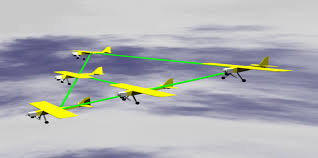
\includegraphics[height =.6\textheight,width=.7\textwidth]{figuras/agentes_vizinhos01.jpeg}
\caption{Observe o sentido das flechas --  e  o foco da missão}
%\label{ag_01}
\end{figure}
    
    
\end{frame}

%-----------------------------------------------------------------------

\begin{frame}
\frametitle{Motivando aos SMAs}

\begin{figure}[!ht]
\centering
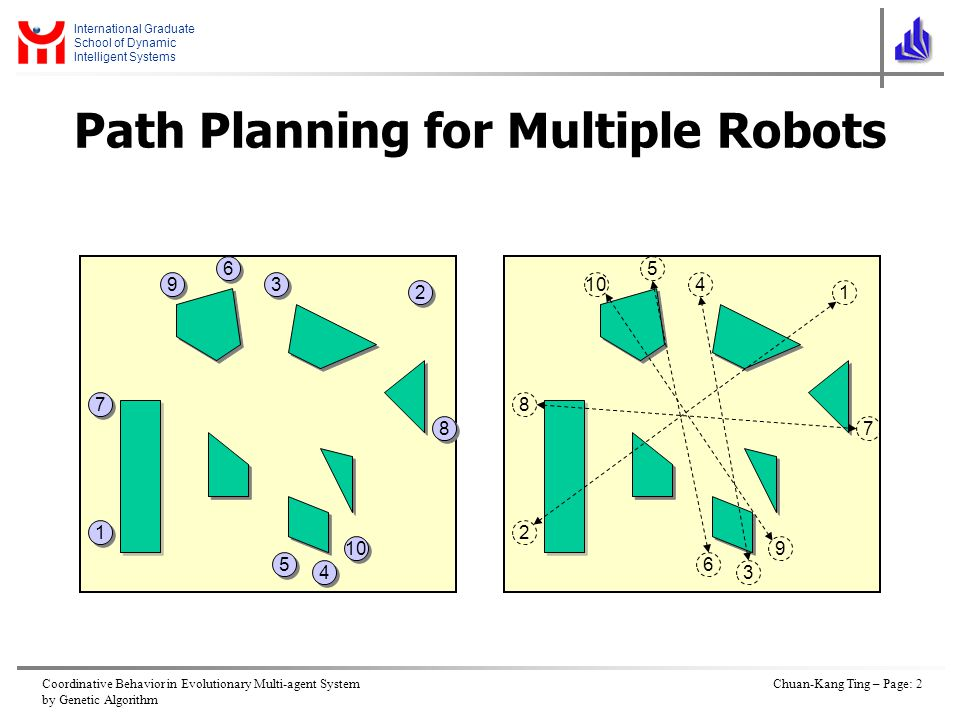
\includegraphics[height =.6\textheight,width=.7\textwidth]{figuras/agentes_vizinhos02.jpeg}
%\caption{Arquitetura clássica}
%\label{ag_01}
\end{figure}
\end{frame}

%-----------------------------------------------------------------------

\begin{frame}

  \frametitle{Motivando aos SMAs}

\begin{figure}[!ht]
\centering
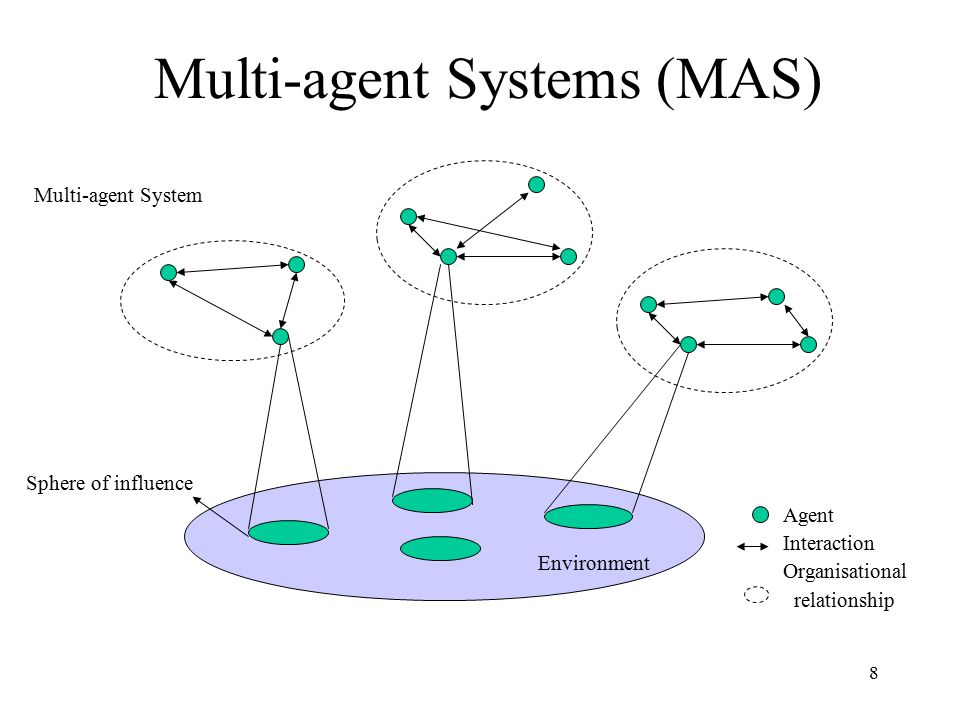
\includegraphics[height =.7\textheight,width=.8\textwidth]{figuras/agentes_vizinhos03.jpeg}
\caption{Visão clássica de SMAs -- comunidade de agentes $\equiv $ SMA}
%\label{ag_01}
\end{figure}
 
\end{frame}
%%%%%%%%%%%%%%%%%%%%%%%%%%%%%%%%%%%%%%%%%%%%%%%%%%%%%%%%%%%%%%%%%


\subsection{Motivação aos SMAs}
\begin{frame} %%%[allowframebreaks=0.9]

\frametitle{Motivação I}
    Projetar e construir sistemas multiagentes é uma tarefa difícil, pois:
 \begin{itemize}
   \pause
   \item Apresenta todos os problemas já conhecidos 
dos sistemas distribuídos e concorrentes.
   \pause
   \item Dificuldades adicionais surgem da flexibilidade 
e complexidade das interações
    \end{itemize}
\end{frame}


%--------------------------------------

\begin{frame}
\frametitle{Problemas de tabuleiro são simples?}
  
  \begin{figure}[!ht]
  \centering
  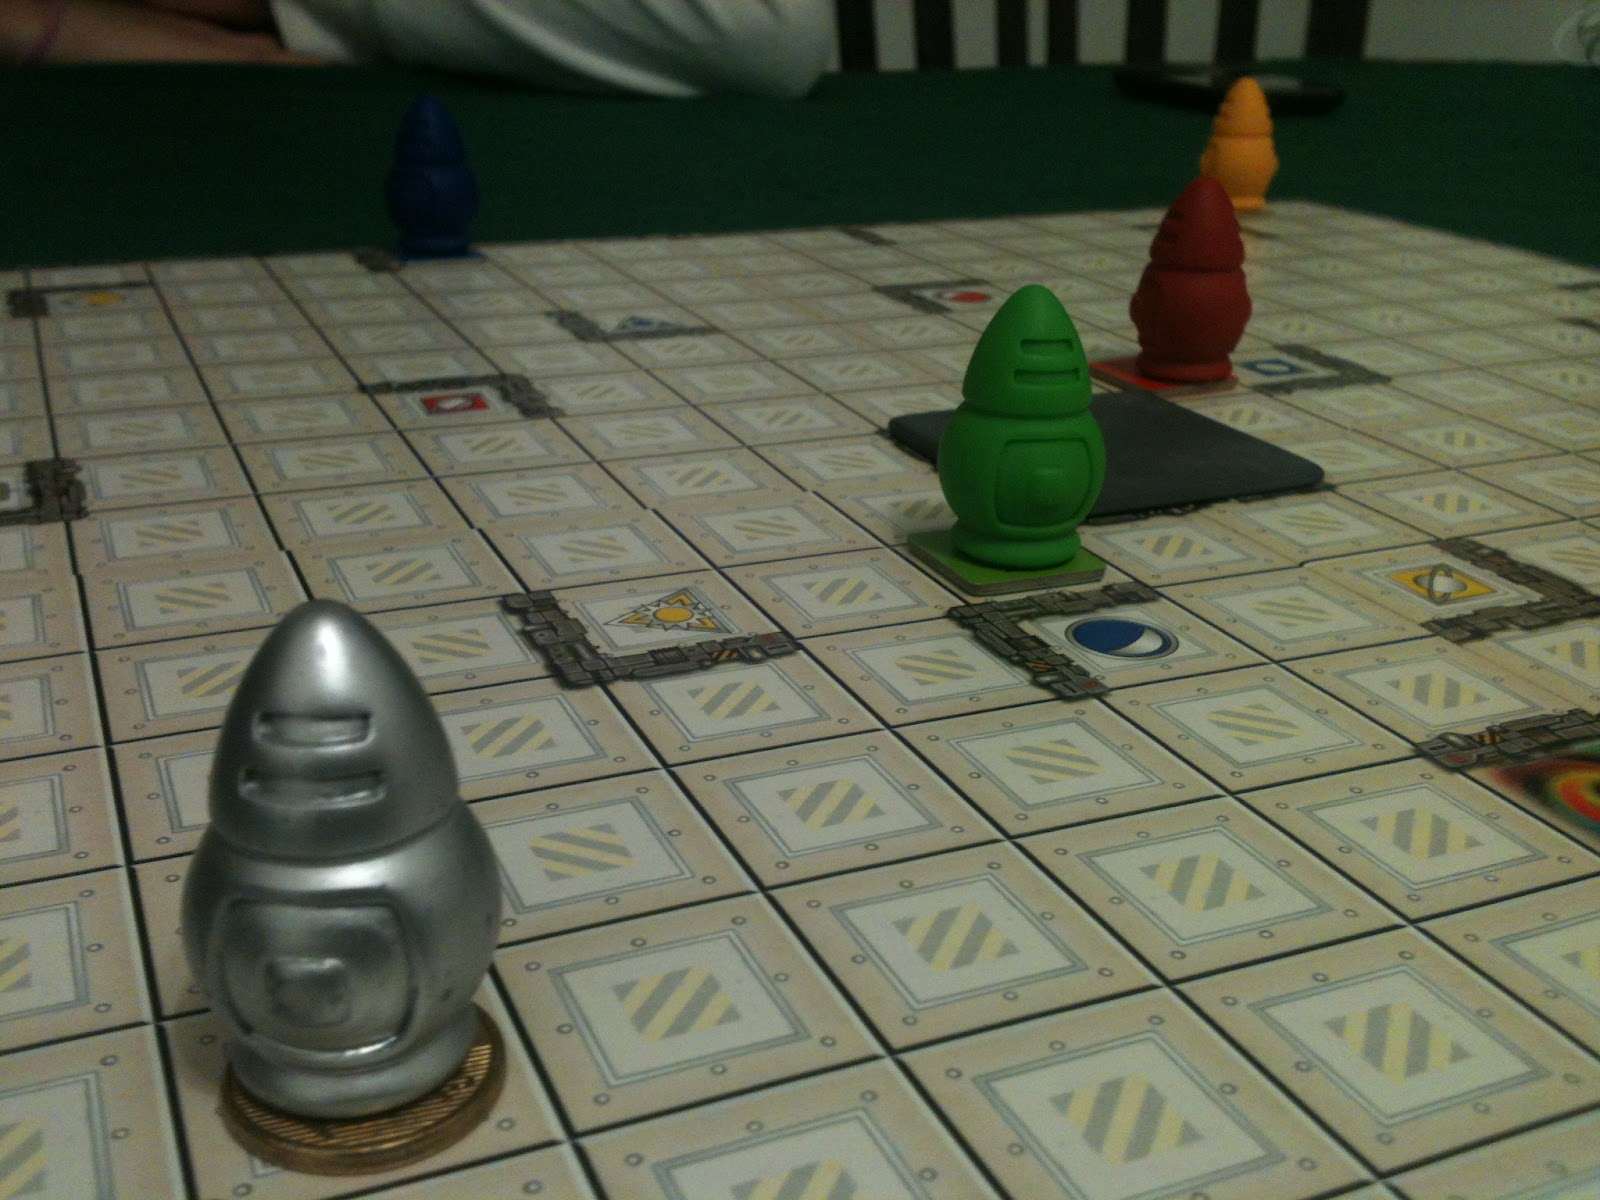
\includegraphics[height =.6\textheight,width=.7\textwidth]{figuras/robos_tabuleiro.jpg}
  \caption{Admita um robo indo de uma posição inicial ($S_0$) há uma final 
  ($S_m$)}
%\label{ag_01}
\end{figure}
   
\end{frame}

%----------------------------------------------------------

\begin{frame}
\frametitle{Exemplificando a complexidade por um DFD com  \textbf{um agente} 
$\times$ \textbf{n-ações}:}
  
  \begin{figure}[!ht]
  \centering
  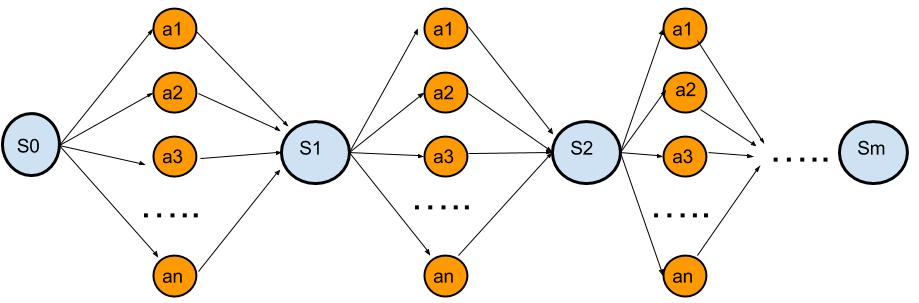
\includegraphics[height =.6\textheight,width=.9\textwidth]{figuras/dfd_simples_acoes.jpg}
  \caption{Complexidade via DFD de um agente $\times $ ações $\equiv $ um estado  inicial ($S_0$) há um estado final ($S_m$)}
%\label{ag_01}
\end{figure}
   
\end{frame}

%----------------------------------------------------------

\begin{frame}
\frametitle{Exemplificando a complexidade por um DFD por \textbf{agentes} $\times$ \textbf{ações}:}
  
  \begin{figure}[!ht]
  \centering
  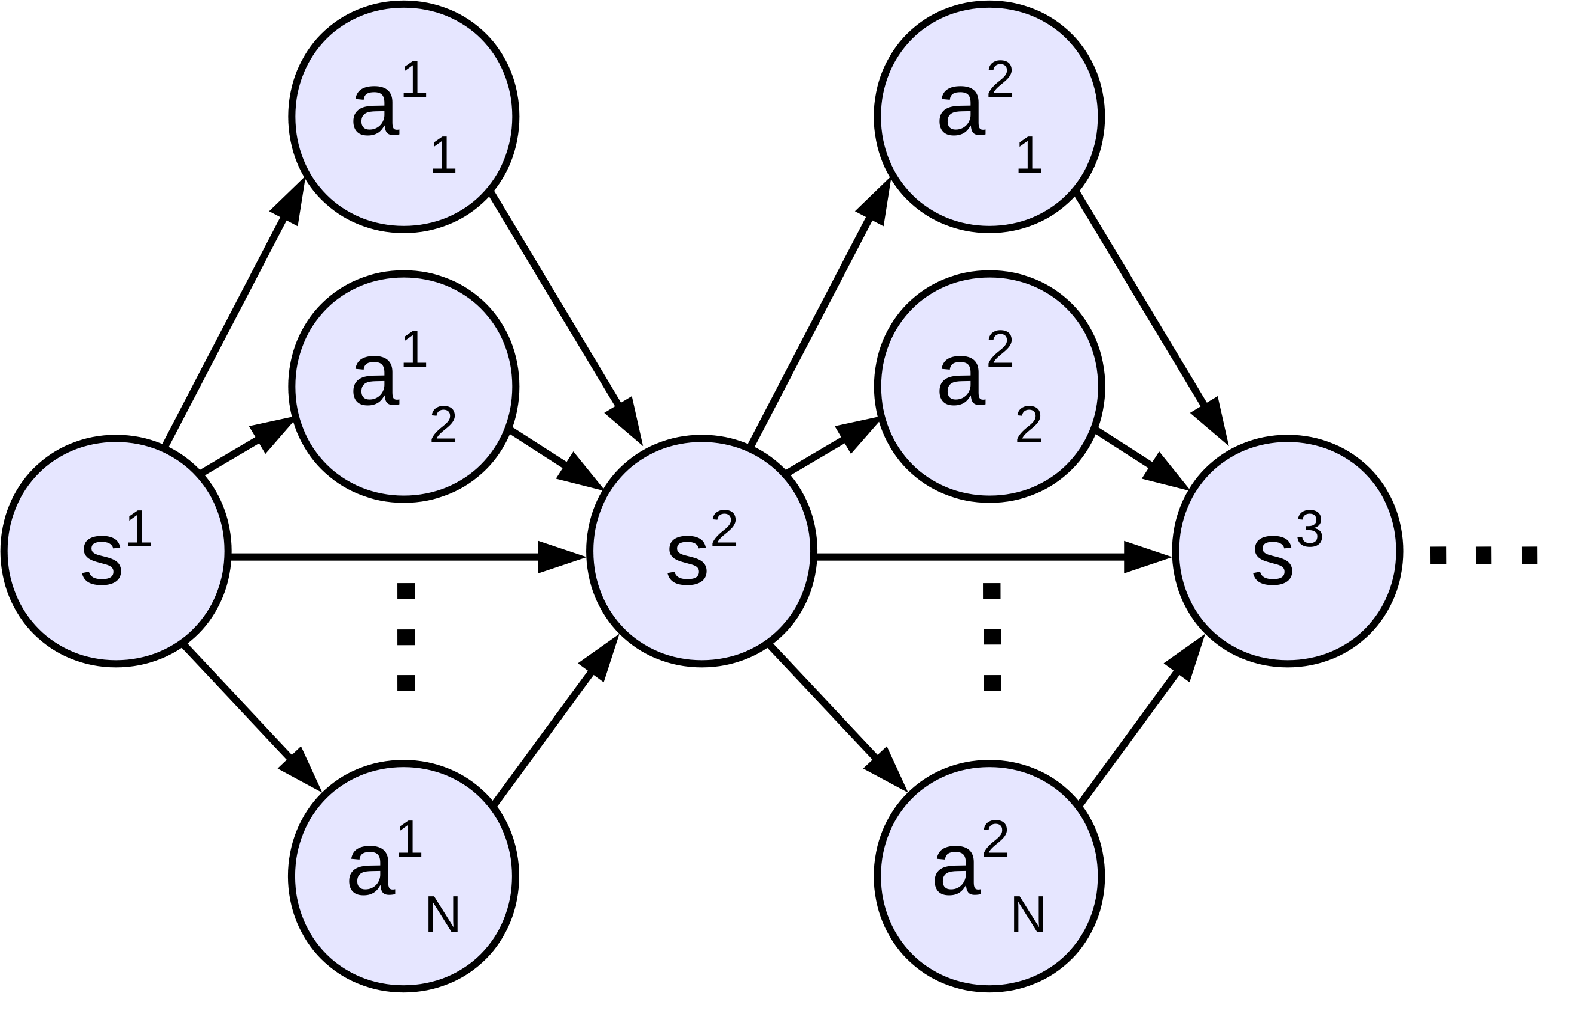
\includegraphics[height =.6\textheight,width=.8\textwidth]{figuras/mudando_estados01.png}
  \caption{Complexidade via DFD de um SMA (agentes) $\times $ ações $\equiv $ um único estado}
%\label{ag_01}
\end{figure}
   
\end{frame}

%----------------------------------------------------------

\begin{frame}

\frametitle{Exercício -- papel e caneta mesmo}
   
\begin{block}{}

  \begin{itemize}
  \item Considere que as ações sejam do tipo um deslocamento de uma célula. 8 direções ou 4?
  \pause
  \item Considere que o robô não vai ficar em ciclos -- passar em estados que já passou -- fácil isto? Como resolver?
  \pause
  
  \item   Para as duas versões acima estime a complexidade dos mesmos em número
  de combinações possíveis de um $S_0$ há um $S_m$.
  \pause
  
   \item Introduza as dimensões do tabuleiro em seus cálculos e refaça-os
  \end{itemize}  
  
\end{block}
   
\end{frame}



%----------------------------------------------------------
\begin{frame}

    \frametitle{Motivação II -- retomando ...}
   Dois principais impedimentos técnicos, pois:
  \begin{itemize}
  \pause
  \item Inexistência de uma metodologia sistemática para 
      claramente especificar e estruturar aplicações SMA.
  \pause
  \item Inexistência de ferramentas e ambientes de 
desenvolvimento de SMA com qualidade industrial.
    
  \end{itemize}

\end{frame}

%----------------------------------------------------------
%%%%%%%%%%%%%%%%%%%%%%%%%%%%%%%%%%%%%%%%%%%%%%%%%%%%%%%%%%%%%%%%%%%%%%%%

\subsection{Os Elementos de SMAs}

\begin{frame}%%%[allowframebreaks=0.9]

 \frametitle{Os Elementos de SMAs}
  
  \begin{block}{O que abordaremos neste curso:}
  
   \begin{description}
  
     \item[Projeto de Agente:] \textbf{\textcolor{red}{... ao longo do curso}}
     
    \item[Ambiente:] \textbf{\textcolor{red}{... ao longo do curso}}
          
   \item[Percepção:] \textbf{\textcolor{red}{... ao longo do curso}}
               
 \item[Controle:] \textbf{\textcolor{red}{... ao longo do curso}}
                    
  \item[Conhecimento:] \textbf{\textcolor{red}{... ao longo do curso}}
                          
  \item[Comunicação:] \textbf{\textcolor{red}{... ao longo do curso}}
          
   \end{description}
  \end{block}    
   
\end{frame}
%-------------------------------------------------



\begin{frame}

\frametitle{Exercício}
   
\begin{figure}[!ht]
\centering
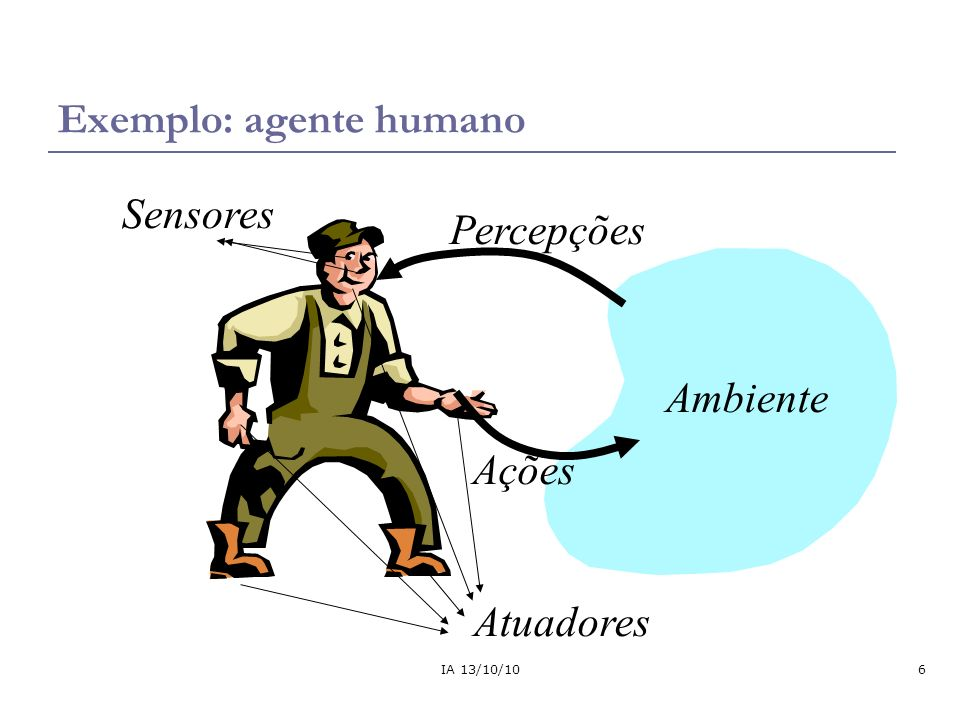
\includegraphics[height =.6\textheight,width=.7\textwidth]{figuras/agente_humano.jpg}
\caption{Exercício: enumere domínios para este agente identificando os itens de SMAs}
%\label{ag_01}
\end{figure}

   
\end{frame}



%%%%%%%%%%%%%%%%%%%%%%%%%%%%
 % cap 1



%%%%%%%%%%%%%%%%%%%%%%%%%%%%%%%%%%%%%%%%%%%%%%%%%%%%%%%%%%%%%%%%%%%%%%%%
\section{Agentes Racionais}


\begin{frame}

\begin{center}
{\huge Capítulo 2 -- Agentes Racionais}
\end{center}

\end{frame}




%--------------------------------------------
\begin{frame} %[allowframebreaks=0.9]

    \frametitle{O que é um Agente?}

\begin{block}{Qualquer entidade (humana ou artificial) que:}
  
  \begin{itemize}
    \item está \textbf{imersa} ou \textbf{situada} em um ambiente (físico, virtual/simulado) 
    \item \textbf{percebe} ou \textbf{sente} seu ambiente através de sensores (ex. câmeras, microfone, teclado, finger, ...)
    \item \textbf{age} sobre ele através de atuadores (ex. vídeo, auto-falante, impressora, braços, ftp, ...)
    \item \textbf{possui objetivos} próprios:
explícitos ou implícitos
    \item \textbf{escolhe} suas ações em função das suas percepções para atingir seus objetivos
  
  \end{itemize}
  
\end{block}

\end{frame}
%--------------------------------------------


%--------------------------------------------
\begin{frame} %[allowframebreaks=0.9]

    \frametitle{Agente Situado x Não-Situado}

    
\begin{figure}[!ht]
\centering
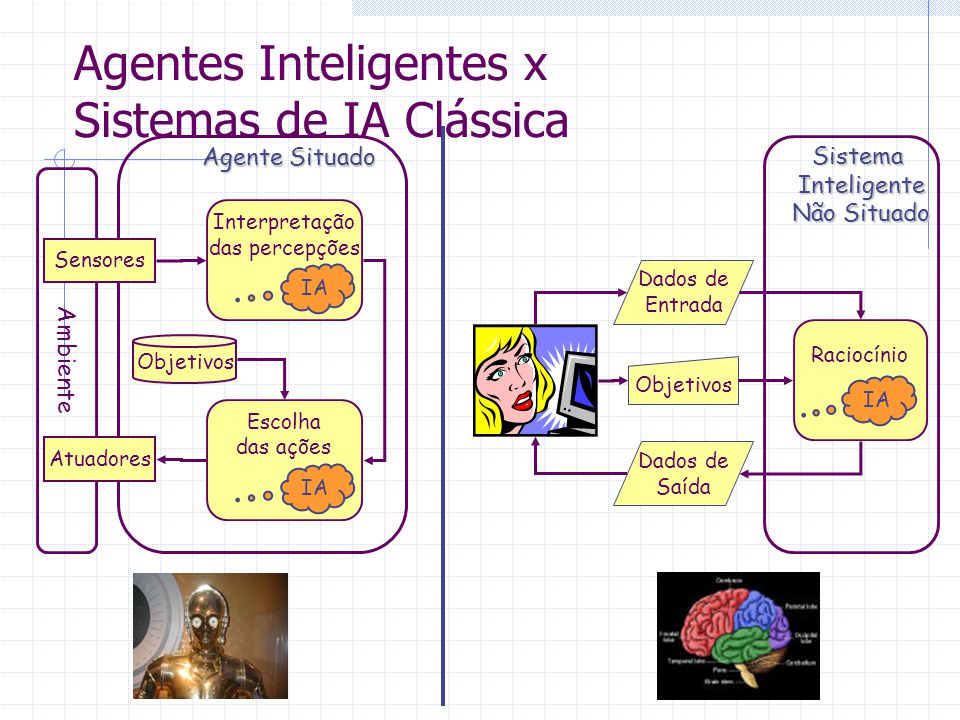
\includegraphics[height =.65\textheight,width=.8\textwidth]{figuras/agente_situado.jpg}
\caption{Agente situado versus a visão clássica de sistemas inteligentes}
%\label{ag_01}
\end{figure}

\end{frame}
%--------------------------------------------


%--------------------------------------------
\begin{frame} %%%[allowframebreaks=0.9]

    \frametitle{O que é um Agente Racional?}

\begin{block}{}
  
 \begin{itemize}
      \item Agente Racional 
 \begin{itemize}
        \item faz a melhor ação possível dado um conjunto de percepções
        \item segue o princípio da racionalidade:\\ 
dada uma seqüência perceptiva, o agente escolhe, segundo seus conhecimentos, 
as ações que melhor satisfazem seu objetivo
      \end{itemize}

\begin{itemize}
  \item Limitações de:\\
  sensores\\
  atuadores\\
  raciocinador (conhecimento, tempo, etc.)
\end{itemize}

    \end{itemize}
  
\end{block}

\end{frame}
%--------------------------------------------



%--------------------------------------------
\begin{frame} [allowframebreaks=0.9]

    \frametitle{Outras propriedades freqüentemente associadas aos Agentes}

 
    \begin{itemize}
      \item Autonomia:\\
raciocínio, comportamento guiado por objetivos ou \\
\textit{reatividade}

\begin{itemize}
  \item Requer máquina de inferência e base de conhecimento
  \item Essencial em sistemas especialistas, controle, robótica, jogos, agentes na internet ...
\end{itemize}
      
    \item Adaptabilidade \& aprendizagem
             
    \begin{itemize}
             
    \item Capacidade de adaptação a situações novas, para as quais não foi fornecido todo o      conhecimento necessário com antecedência 

     \item Duas implementações: sistema com  
           aprendizagem 
           e/ou programação declarativa
  
     \item Essencial em agentes na internet, interfaces amigáveis ...
   
    \end{itemize}
             
             
    \item Comunicação \& Cooperação (sociabilidade)
         \begin{itemize}
          \item  Protocolos padrões de comunicação, cooperação, negociação
          \item  Raciocínio autônomo sobre crenças e confiabilidade
          \item  Arquiteturas de interação social entre agentes
                      
         \end{itemize}
         
                
    \item Personalidade
    
    \begin{itemize}
      \item IA + modelagem de atitudes e emoções (computação afetiva)
      \item Essencial em entretenimento digital, realidade virtual, interfaces amigáveis ... 
    \end{itemize}
    
    \item Continuidade temporal (persistência)
    \begin{itemize}
      \item Requer interface com sistema operacional e banco de dados
    \item Essencial em filtragem, monitoramento, controle, ...
    \end{itemize}
    
    
 \item Mobilidade (caso internet)
  \begin{itemize}
     \item Requer itens como:
     \begin{enumerate}
       \item Interface com rede
       \item Protocolos de segurança
       \item Suporte a código móvel
     \end{enumerate}

    \item Essencial em agentes de exploração da internet, ...
         
     \end{itemize}      
                  
    \end{itemize}
 
\end{frame}
%--------------------------------------------

%--------------------------------------------
\begin{frame} %[allowframebreaks=0.9]

 \frametitle{Exercício}
    
\begin{figure}[!ht]
\centering
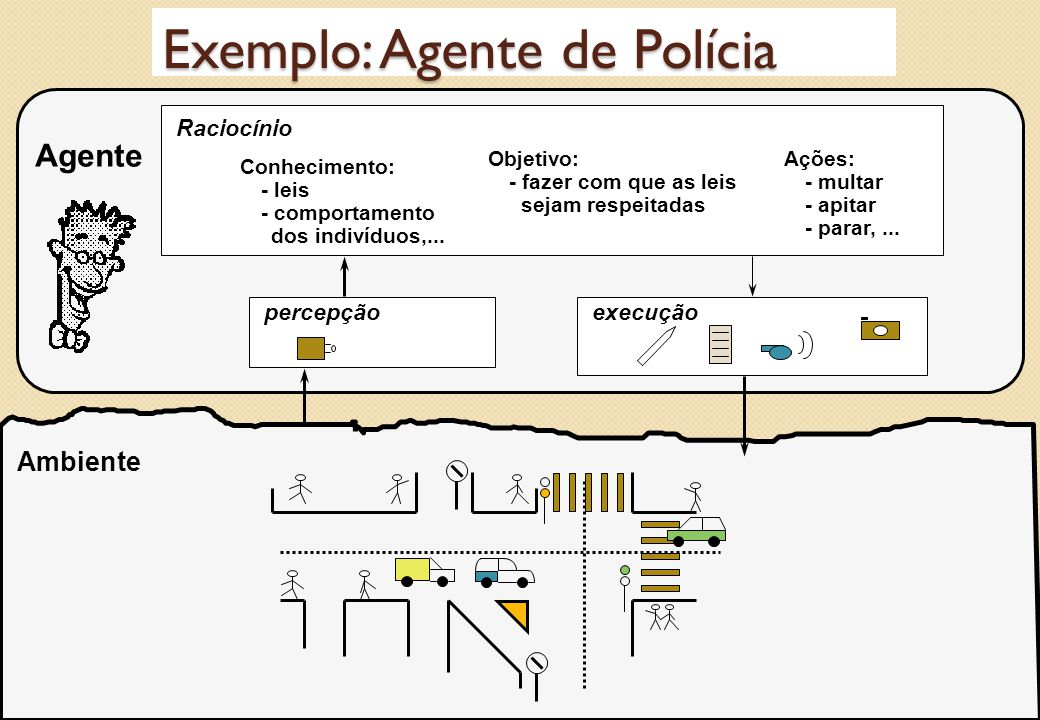
\includegraphics[height =.6\textheight,width=.8\textwidth]{figuras/agente_policial.jpg}
\caption{Exercício: enumere as características citadas a este exemplo -- ao final do capítulo este exercício deve ser rediscutido}
\label{agente_policial}
\end{figure}

\end{frame}
%--------------------------------------------



\subsection{Tipos de Agentes}
\begin{frame} [allowframebreaks=0.9]
\frametitle{Tipos de Agentes}

Em geral os agentes encontram-se em  dois grupos (2 classes):

\begin{description}

 \item[Agentes Reflexivos:] geralmente são agentes simples, escolhem suas 
 ações baseados \textbf{exclusivamente} nas percepções que têm do ambiente. 
 Normalmente possuem uma representação do conhecimento implícita  no código, por não  possuirem  memória, não tem histórico dos fatos  e das ações que executou.
 
 \begin{itemize}
   \item Nota: nestes slides, ora são chamados de  \textit{reativos}
   
   \item Na 3a. versão do livro do Russel e Norvig -- utiliza-se o termo \textit{reflexivo}
   
   \item Ver fundamentação biológica para este termo -- está correta
   
   \item Nos primórdios da área: o termo é \textit{reativo} 
   
 \end{itemize}

 
\newpage

  \item[Agentes Cognitivos:]  têm uma representação simbólica explícita do seu ambiente, no qual eles podem argumentar e predizer eventos futuros. Estes são dirigidos por intenções, isto é, por metas explícitas que conduzem seu comportamento e os tornam capazes de escolher entre possíveis ações. 
  Engloba as características: \textit{\textcolor{blue}{percepção, ação, comunicação,  representação, 
  motivação, deliberação, raciocínio e aprendizagem}}. 

\end{description}

\end{frame}
%--------------------------------------------------------------------------
\begin{frame}

  \frametitle{Arquitetura clássica de um agente reflexivo}
    
\begin{figure}[!ht]
\centering
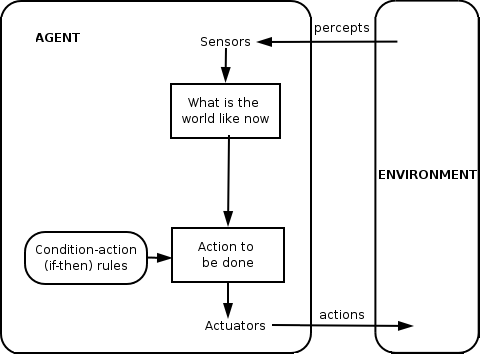
\includegraphics[width=.6\textwidth]{figuras/agente_reflexivo.png}
\caption{Arquitetura clássica -- reflexivo}
\label{ag_01}
\end{figure}
    
\end{frame}

%--------------------------------------------------------------------------
\begin{frame}

  \frametitle{Arquitetura clássica de um agente cognitivo (\textit{que aprende algo!}}
    
\begin{figure}[!ht]
\centering
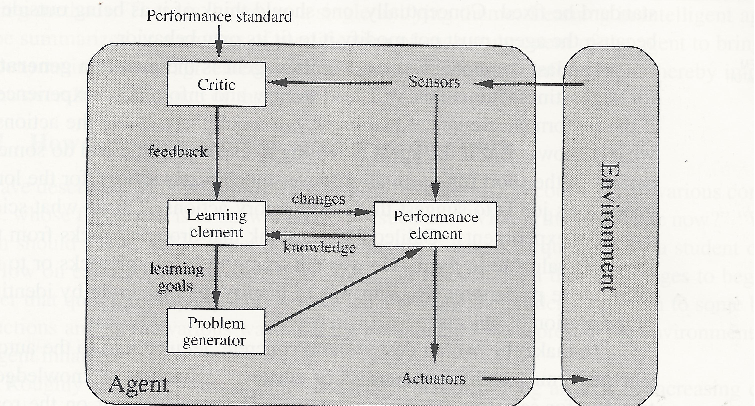
\includegraphics[height =.6\textheight,width=.7\textwidth]{figuras/agente_aprendizagem.pdf}
\caption{Arquitetura clássica -- agente cognitivo com aprendizagem}
\label{ag_02}
\end{figure}
    
\end{frame}



%--------------------------------------------
\subsection{Arquiteturas de Agentes}
\begin{frame} %[allowframebreaks=0.9]

\frametitle{Arquiteturas ou Modelos de Agentes}

\begin{block}{Destes 2 grupos(reflexivo e cognitivo), delinea-se algumas arquiteturas:}
  
    \begin{itemize}
      \item Agente tabela (menos complexo -- mais baixo-nível $\downarrow $)
      \item Agente reativo
      \item Agente reativo com estado interno 
      \item Agente baseado em objetivos (com \textit{alguma} cognição)
      \item Agente otimizador
      \item Agente adaptativo (mais complexo -- mais alto-nível $\uparrow $)
    \end{itemize}
  
\end{block}

\end{frame}
%--------------------------------------------


%--------------------------------------------

\begin{frame} %[allowframebreaks=0.9]

    \frametitle{Genericamente todos seguem algo como:}

Um agente pode ser visto como um \textcolor{red}{\texttt{mapeamento}}: 
\textbf{seqüência e/ou fusão de percepções $\Rightarrow$  ação}

\begin{figure}[!ht]
  \centering
  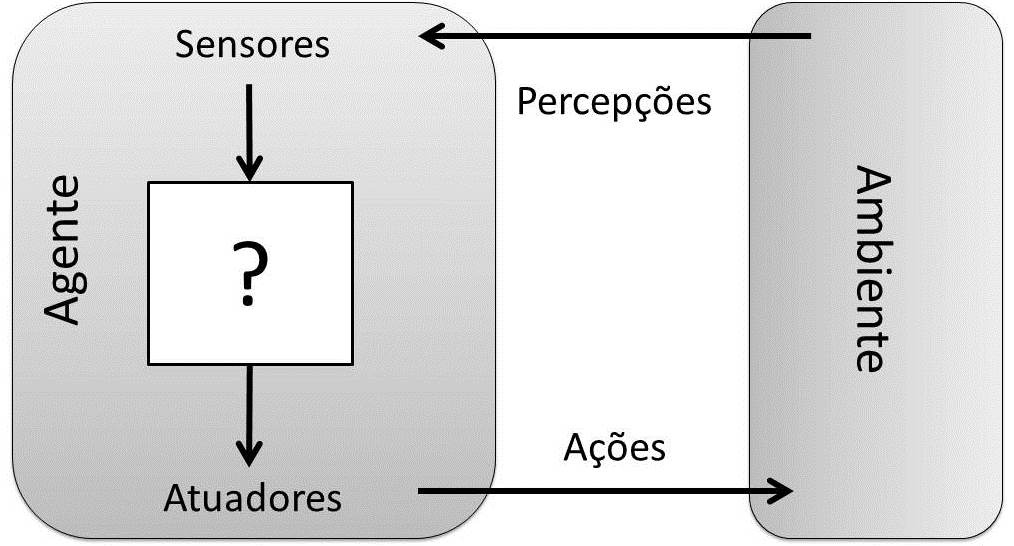
\includegraphics[height =.5\textheight,width=.7\textwidth]{figuras/agente_generico.jpg}
  \caption{Agente Genérico}
%\label{ag_01}
\end{figure}
%--------------------------------------------
\end{frame}

%--------------------------------------------

\begin{frame} %[allowframebreaks=0.9]

    \frametitle{Agente Tabela – é mesmo um agente racional?}

\begin{figure}[!ht]
  \centering
  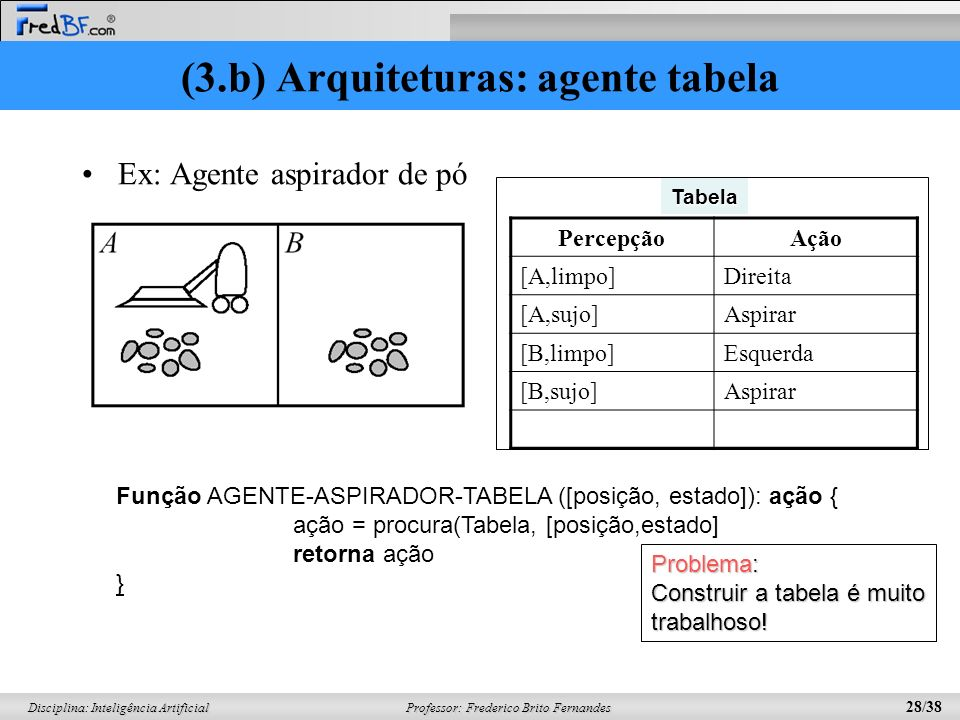
\includegraphics[height =.6\textheight,width=.7\textwidth]{figuras/agente_tabela.jpg}
  \caption{Agente Tabela -- seguem os \textit{copyrights}}
%\label{ag_01}
\end{figure}

\end{frame}
%--------------------------------------------



%--------------------------------------------

\begin{frame} %[allowframebreaks=0.9]

    \frametitle{Agente Tabela}

\begin{itemize}
  \item Limitações
  \begin{itemize}
    \item Mesmo problemas simples requerem tabelas muito grandes 
Ex. jogo de xadrez $30^{100}$
    \item Nem sempre é possível, por ignorância ou questão de tempo, construir a tabela 
    \item  Não há autonomia nem flexibilidade
    
    \item Este \textit{infeliz} entra em pane se o conhecimento  não estiver descrito na tabela (inferior há uma regra \textit{if-then})
    
  \end{itemize}
  
  \item Ambiente
\begin{itemize}
  \item do tipo acessível:  determinista, episódico, 
   estático, discreto e minúsculo!
   
\end{itemize}
  
\end{itemize}
\end{frame}
%--------------------------------------------



\begin{frame} %[allowframebreaks=0.9]

\frametitle{Agente Reativo}

\begin{figure}[!ht]
  \centering
  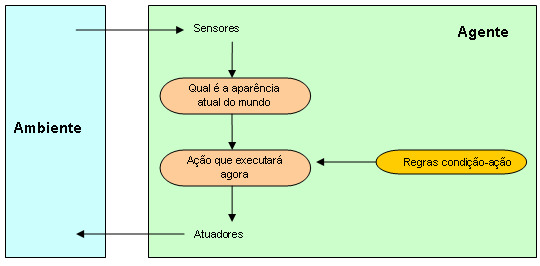
\includegraphics[height =.6\textheight,width=.7\textwidth]
  {figuras/agente_reativo.jpg}
  \caption{Agente Reativo -- seguem os \textit{copyrights}}
%\label{ag_01}
\end{figure}

\end{frame}
%--------------------------------------------



%--------------------------------------------

\begin{frame} %[allowframebreaks=0.9]

    \frametitle{Agente Reativo}

\begin{itemize}
  \item Vantagens e desvantagens
  \begin{itemize}
    \item Regras condição-ação: representação inteligível, modular e eficiente\\ 
Ex: \texttt{Se velocidade $>$ 60 então multar}
   \item Não pode armazenar uma seqüência perceptiva, pouca autonomia
  \end{itemize}
  
  \item Ambientes
\begin{itemize}
  \item Reflexo imprescindível em ambientes dinâmicos 
  \item Acessível, episódico, pequeno 
\end{itemize}
  
\end{itemize}
\end{frame}
%--------------------------------------------


\begin{frame} %[allowframebreaks=0.9]

 \frametitle{Agente reativo com estado interno}

\begin{figure}[!ht]
  \centering
  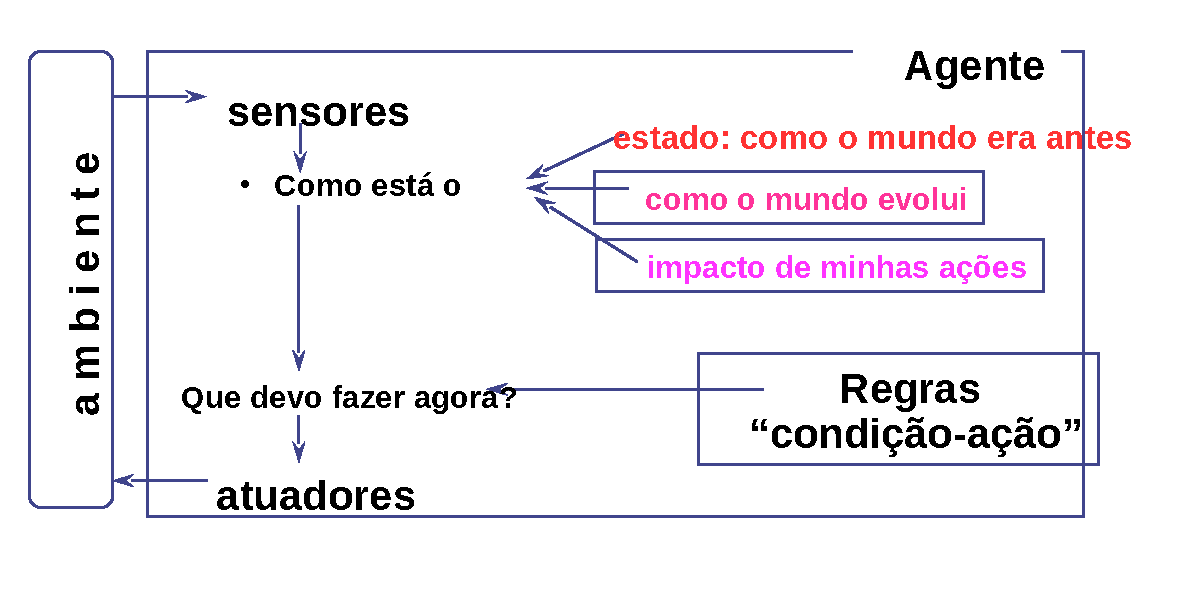
\includegraphics[height =.6\textheight,width=.7\textwidth]
  {figuras/agente_reativo_com_estado_interno.pdf}
  \caption{Agente reativo com estado interno -- seguem os \textit{copyrights}}
%\label{ag_01}
\end{figure}

\end{frame}
%--------------------------------------------



%--------------------------------------------

\begin{frame} %[allowframebreaks=0.9]

    \frametitle{Agente reativo com estado interno}

\begin{itemize}
  \item Desvantagens
  \begin{itemize}
    \item pouca autonomia

   \item não tem objetivo, não encadeia regras
   
   \item melhorar a figura .... \textit{como está o mundo agora?}
  \end{itemize}
  
  \item Ambientes
\begin{itemize}
  \item determinista e pequeno 
  \item Ex. Tamagotchi -- sucesso 
\end{itemize}
  
\end{itemize}
\end{frame}
%--------------------------------------------


\begin{frame} %[allowframebreaks=0.9]

 \frametitle{Agente baseado em objetivo}

\begin{figure}[!ht]
  \centering
  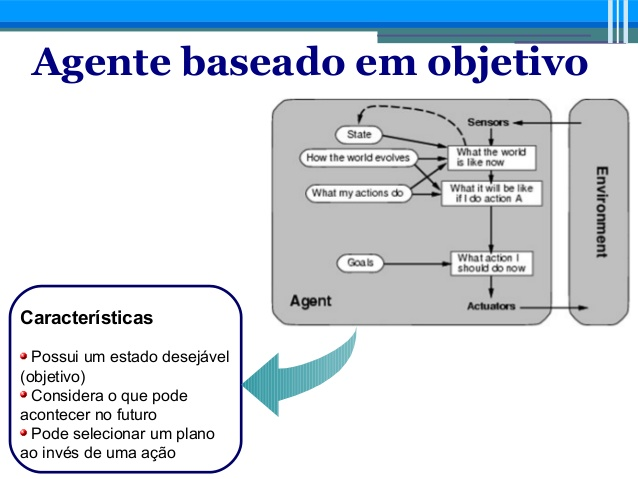
\includegraphics[height =.7\textheight,width=.7\textwidth]
  {figuras/agente_baseado_em_objetivo.jpg}
  \caption{Agente baseado (orientado) em objetivo -- seguem os \textit{copyrights}}
%\label{ag_01}
\end{figure}

\end{frame}
%--------------------------------------------



%--------------------------------------------

\begin{frame} %[allowframebreaks=0.9]

    \frametitle{Agente baseado em objetivo}

\begin{itemize}
  \item Vantagens e desvantagens

  \begin{itemize}
    \item Mais complicado e ineficiente,  porém mais flexível, autônomo
    \item Não trata objetivos conflitantes
  \end{itemize}
  
  \item Ambientes

\begin{itemize}
  \item determinista 
  \item Ex.ex.: xeque-mate no xadrez
\end{itemize}
  
\end{itemize}
\end{frame}
%--------------------------------------------

%--------------------------------------------


\begin{frame} %[allowframebreaks=0.9]

 \frametitle{Agente otimizador (\textit{utility based})}

\begin{figure}[!ht]
  \centering
  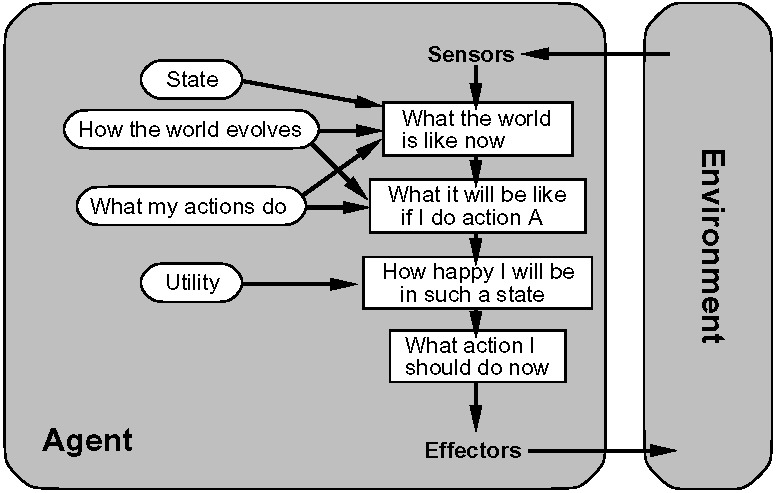
\includegraphics[height =.6\textheight,width=.7\textwidth]
  {figuras/agente_otimizador.jpg}
  \caption{Agente otimizador -- seguem os \textit{copyrights}}
%\label{ag_01}
\end{figure}

\end{frame}

%----------------------------------------------------------------------------------------

\begin{frame} %[allowframebreaks=0.9]

    \frametitle{Agente otimizador}

\begin{itemize}
  \item Ambiente: sem restrição
  
  \item Desvantagem: não  tem adaptabilidade
  
  \item Ex. \texttt{alguns} motoristas do Brasil\\
    Segurança e velocidade – conflito!
  
\end{itemize}
\end{frame}
%--------------------------------------------


%--------------------------------------------


\begin{frame} %[allowframebreaks=0.9]

 \frametitle{Agente que aprende (\textit{learning agent})}

\begin{figure}[!ht]
  \centering
  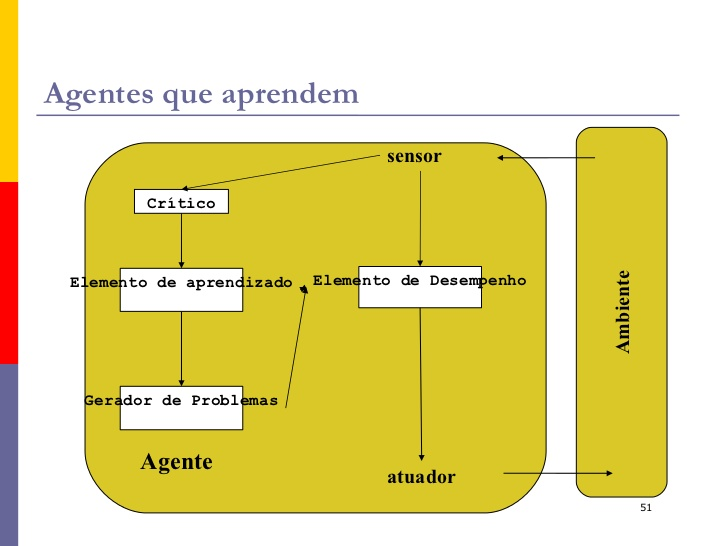
\includegraphics[height =.6\textheight,width=.7\textwidth]
  {figuras/agentes_que_aprendem.jpg}
  \caption{Agente que aprende -- seguem os \textit{copyrights}}
%\label{ag_01}
\end{figure}

\end{frame}
%--------------------------------------------



%--------------------------------------------

\begin{frame} %[allowframebreaks=0.9]

    \frametitle{Agente que aprende}

\begin{itemize}
  \item Ambiente: sem restrição
  
  \item Vantagem:  tem adaptabilidade (aprende)
  
  \item Ex.  motoristas em um GPS
  
\end{itemize}
\end{frame}
%--------------------------------------------



\section{Construindo de Agentes Racionais}

\begin{frame}%%[allowframebreaks=0.9]

% \frametitle{Uma medida de eficácia para estes agentes (racionais)?}
   \frametitle{Metodologia de desenvolvimento destes agentes racionais}
  \begin{block}{\textbf{PEAS} = Peformance, Ambiente (\textit{Enviroment}), Ação e Sensores}
  
   \begin{description}
  
     \item[Peformance:] como ter um indicativo de sucesso
     
    \item[Ambiente:]  cuidado deve ser sempre 
especificar o ambiente
          
   \item[Ação:] o que vai fazer?
                          
  \item[Sensores:] o que vai perceber?

  \item[Outros:] agentes da comunidade (falta isto na construção de agentes), ou seja um SMA!

          
   \end{description}
  \end{block}    
   
\end{frame}


%--------------------------------------------


\begin{frame} %[allowframebreaks=0.9]

 \frametitle{Exemplo ao avaliar (projetar ...) SMAs}

\begin{figure}[!ht]
  \centering
  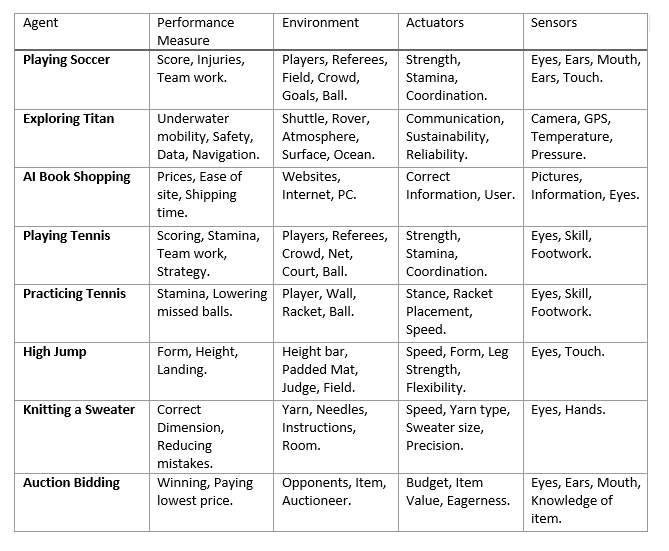
\includegraphics[height =.7\textheight,width=.8\textwidth]
  {figuras/PEAS01.png}
  \caption{Um bom exercício para reflexão -- seguem os \textit{copyrights}}
%\label{ag_01}
\end{figure}

\end{frame}
%--------------------------------------------

%--------------------------------------------

\begin{frame} %[allowframebreaks=0.9]

 \frametitle{Exemplo ao avaliar (projetar ...) SMAs}

\begin{figure}[!ht]
  \centering
  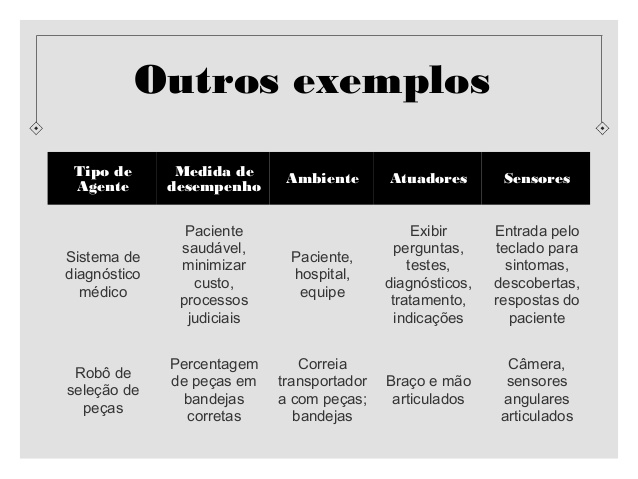
\includegraphics[height =.7\textheight,width=.8\textwidth]
  {figuras/PEAS02.jpg}
  \caption{Um bom exercício para reflexão -- seguem os \textit{copyrights}}
%\label{ag_01}
\end{figure}

\end{frame}

\begin{frame} %[allowframebreaks=0.9]

 \frametitle{Volte ao exemplo do agente policial -- ver figura \ref{agente_policial}}

\begin{itemize}
  \item Quem é seu ambiente?
  \item Quem são seus sensores?
    \item Quem são seus atuadores?
    \item Qual é o seu mecanismo de raciocínio?
    \item Há outros agentes?
    \item Como é o seu ambiente (discreto, episódico..... -- ver características do livro do Norvig--Russel)?
    \item Sua interação com o ambiente?
    \item Há outros agentes? Quais? Comunidades?
\end{itemize}


\end{frame}

%-----------------------------------------------------------

\begin{frame} %[allowframebreaks=0.9]

 \frametitle{Resumo do capítulo}

\begin{enumerate}
  \item Vocabulário
  \item Uma gama de agentes ...
    \begin{itemize}
    \item Dos reativos: os mais simples, e quando numa comunidade são todos iguais
    \item Aos cognitivos: os mais complexos, e quando numa comunidade apresentam
    uma metáfora social de humanos
  \end{itemize}
  
  \item Como iniciar um desenvolvimento de SMAs 
  
  \item Falta: porque soluções de SMAs são atrativas
    \item Falta: diferença de SMAs com RDPs
    \item Falta: Coordenação etc
        \item Falta: Planejamento etc
    
\end{enumerate}


\end{frame}
 % cap 2

\section{IAD $\supseteq $ RDP $\times$ SMA }
%------------------------------------------------------------------------
\begin{frame}

\begin{center}
{\huge Capítulo 3 -- IAD $\supseteq $ RDP $\times$ SMA }
\end{center}

\end{frame}

%------------------------------------------------------------------------
\begin{frame} %[allowframebreaks=0.9]


\frametitle{O que vai ter neste capítulo}

\begin{itemize}
  \item Mais conceitos sobre SMA dentro da IAD ... vantagens etc
  \item Quando a RDP é mais interessante (e quando não é)
  \item Vantagens da SMA (e desvantagens com relação a RDP)
\end{itemize}


\end{frame}

%------------------------------------------------------------------------


\begin{frame} %[allowframebreaks=0.9]


\frametitle{Porque distribuir?}

\begin{itemize}
  \item Sistemas em geral são distribuídos \textbf{funcionalmente}
  \pause
  \begin{itemize}
    \item Devido uma especificação (a necessidade ou requisitos)
    \item Devido uma especialização
    \item Dividir e diminuir a complexidade $\rightarrow$ decompor o problema
    
  \end{itemize}

  \pause
  \item Sistemas em geral são distribuídos \textbf{fisicamente}
  \pause  
  \item Finalmente, na \textbf{resolução de problemas} (em geral): 
  há alguns cuja solução é inerentemente distribuída ou 
  fica mais fácil distribuindo!
  

\end{itemize}


\end{frame}
%------------------------------------------------------------------------

\begin{frame} %[allowframebreaks=0.9]

  \frametitle{Motivando o \textit{distribuído}}
        
\begin{figure}[!ht]
\centering
%\includegraphics{}
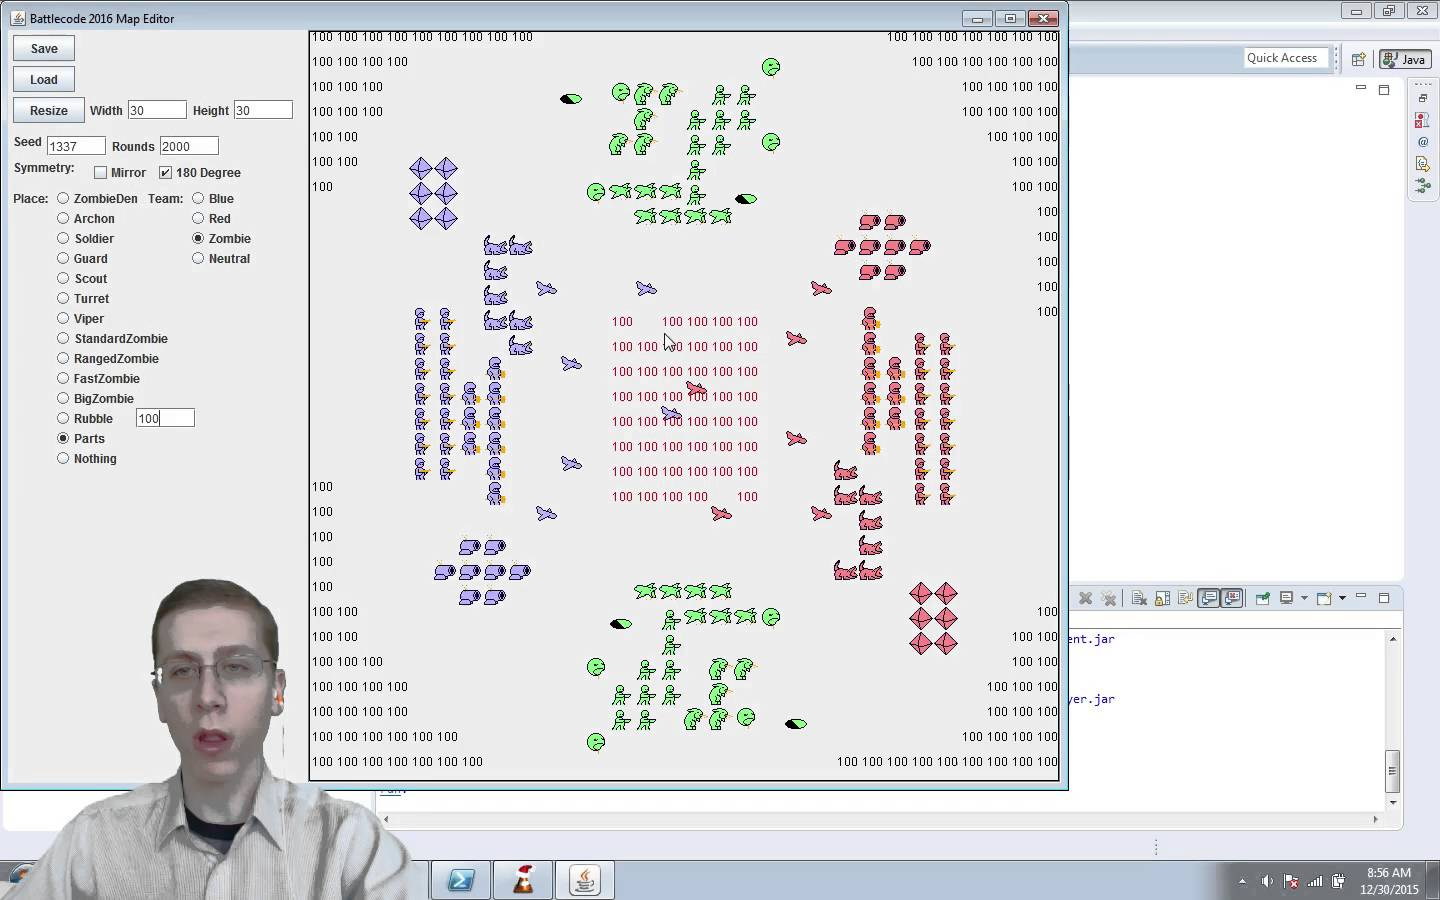
\includegraphics[height =.6\textheight,width=.7\textwidth]{figuras/DAI_motivation01.jpg}
\caption{Ações paralelas, distribuídas, concorrentes ... e tudo coordenado?}
%\label{ag_01}
\end{figure}
    
\end{frame}

%------------------------------------------------------------------------

\begin{frame} %[allowframebreaks=0.9]

  \frametitle{Motivando o \textit{distribuído}}
        
\begin{figure}[!ht]
\centering
%\includegraphics{}
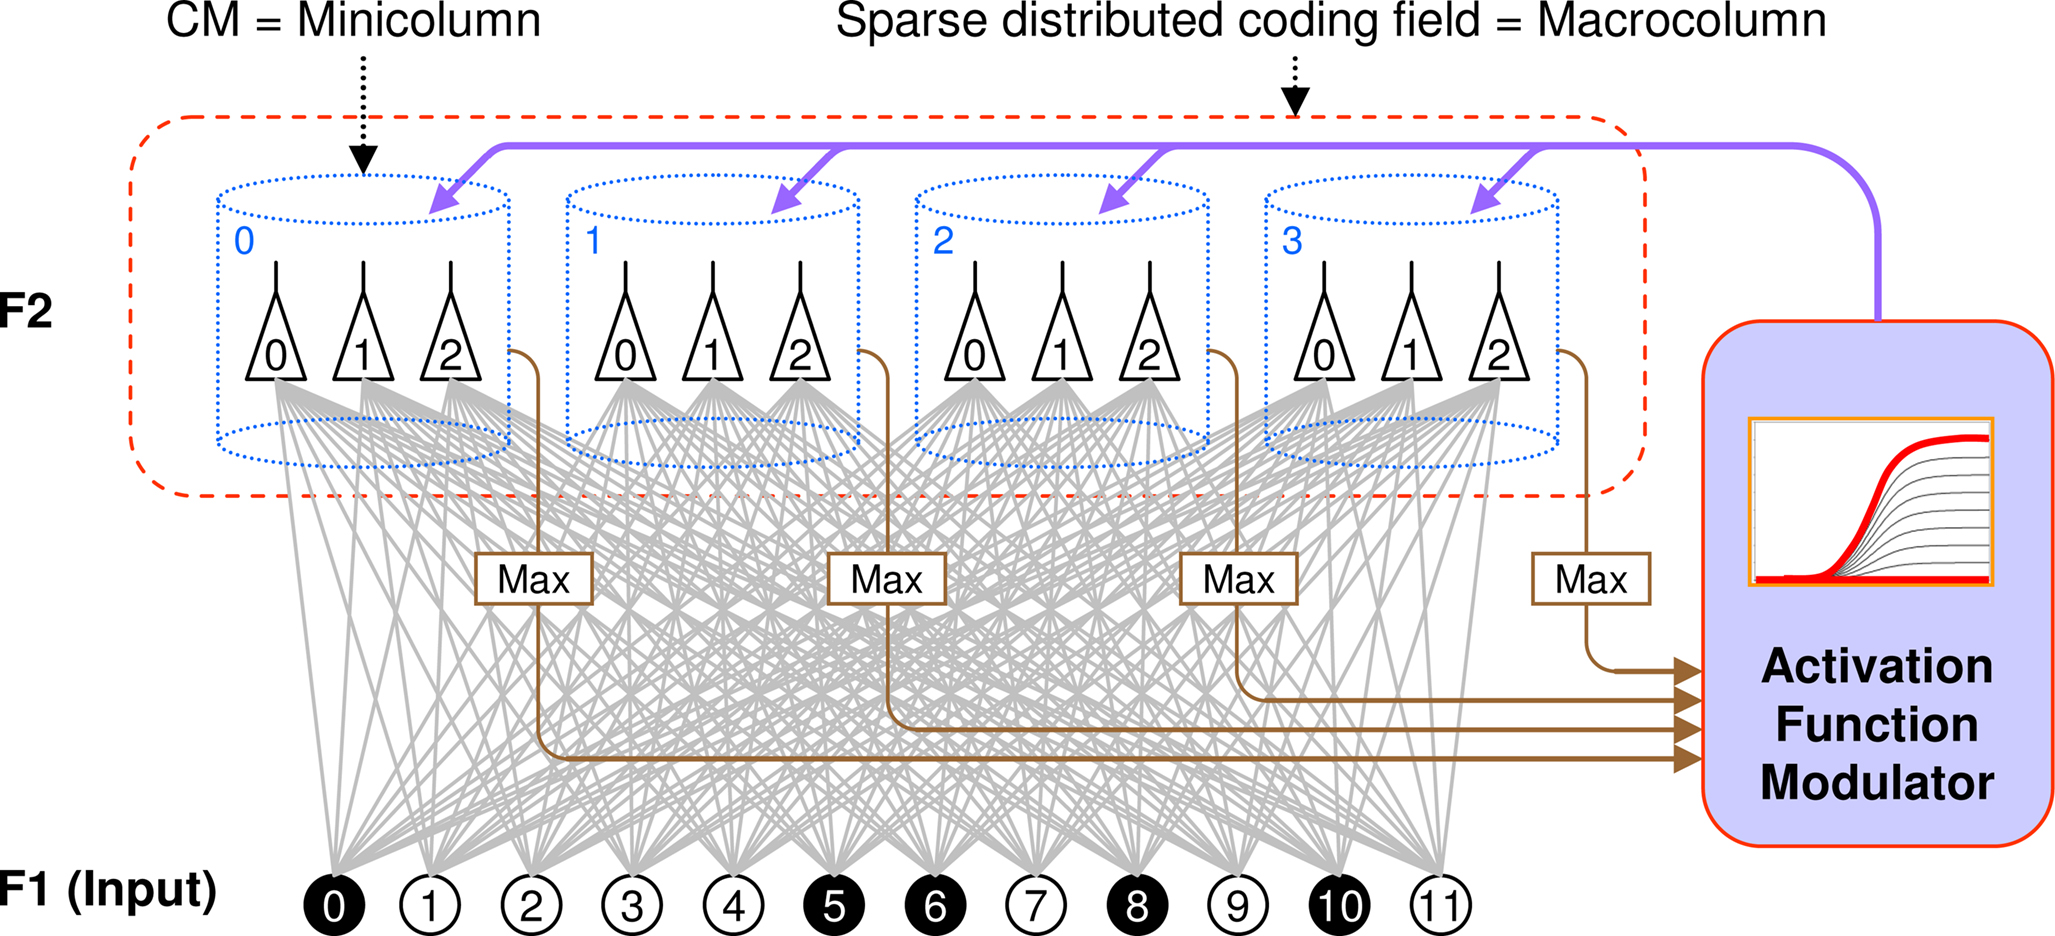
\includegraphics[height =.6\textheight,width=.8\textwidth]{figuras/DAI_motivation02.jpg}
\caption{Mapeando funções via RN -- representações funcionais -- cérebro}
%\label{ag_01}
\end{figure}
    
\end{frame}

%------------------------------------------------------------------------

\begin{frame} %[allowframebreaks=0.9]

  \frametitle{Motivando o \textit{distribuído}}
        
\begin{figure}[!ht]
\centering
%\includegraphics{}
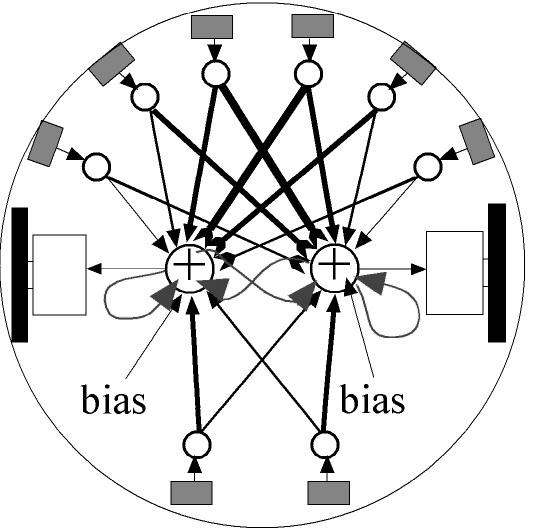
\includegraphics[height =.5\textheight,width=.4\textwidth]{figuras/DAI_motivation03.jpg}
\caption{Robô: mapeando sensores funcionais em atividades motoras $\Rightarrow$ Inspiração 100 \% na entomologia -- ver robôs de Braitenberg}
%\label{ag_01}
\end{figure}
    
\end{frame}




%------------------------------------------------------------------------

\begin{frame} %[allowframebreaks=0.9]

  \frametitle{Arquitetura de  Braitenberg -- 01}
        
\begin{figure}[!ht]
\centering
%\includegraphics{}
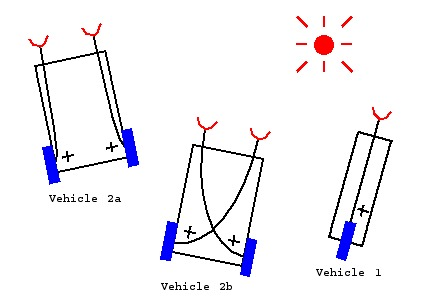
\includegraphics[height =.5\textheight,width=.6\textwidth]{figuras/braitember01.jpg}
\caption{Robôs de Braitenberg}
%\label{ag_01}
\end{figure}
    
\end{frame}
%------------------------------------------------------------------------

\begin{frame} %[allowframebreaks=0.9]

  \frametitle{Arquitetura de  Braitenberg -- 02}
        
\begin{figure}[!ht]
\centering
%\includegraphics{}
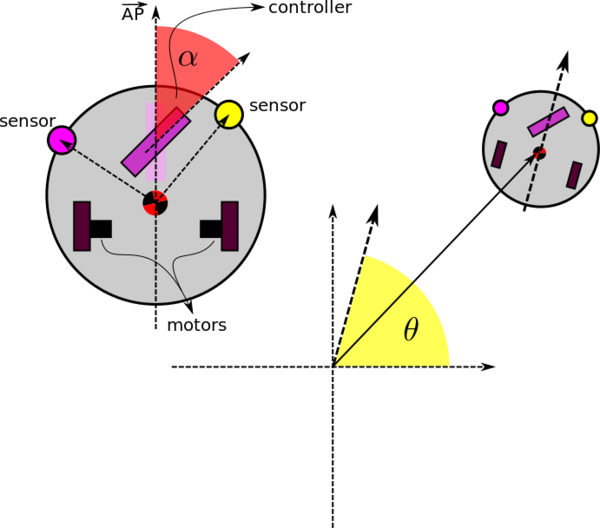
\includegraphics[height =.55\textheight,width=.5\textwidth]{figuras/braitember02.jpg}
\caption{Robôs de Braitenberg}
%\label{ag_01}
\end{figure}
    
\end{frame}
%------------------------------------------------------------------------

\begin{frame} %[allowframebreaks=0.9]

  \frametitle{Arquitetura de  Braitenberg -- 03}
        
\begin{figure}[!ht]
\centering
%\includegraphics{}
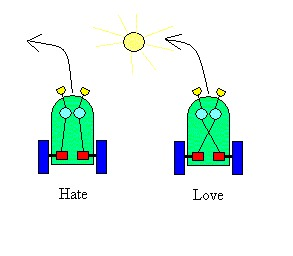
\includegraphics[height =.55\textheight,width=.54\textwidth]{figuras/braitember03.jpg}
\caption{Robôs de Braitenberg -- Inteligência = Comportamento Complexo}
%\label{ag_01}
\end{figure}
    
\end{frame}



%------------------------------------------------------------------------

\begin{frame} %[allowframebreaks=0.9]

  \frametitle{Há muito cálculo \textit{distribuído}, como os processos mentais:}
        
\begin{figure}[!ht]
\centering
%\includegraphics{}
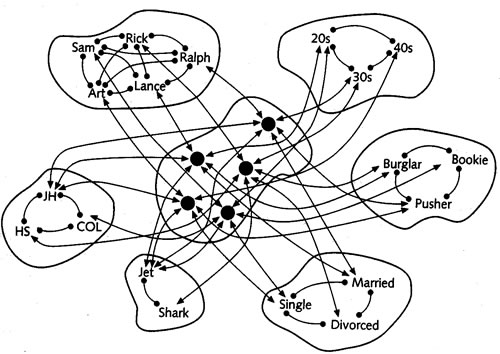
\includegraphics[height =.6\textheight,width=.8\textwidth]{figuras/processamento_mental_01.jpg}
%\caption{Robo: mapeando sensores funcionais em atividades motoras $\Rightarrow$ Inspiração 100 \% na entomologia}
%\label{ag_01}
\end{figure}
    
\end{frame}



%------------------------------------------------------------------------


\begin{frame} %[allowframebreaks=0.9]


\frametitle{Motivando a distribuição:}

\begin{itemize}
  \item Porque o problema é fisicamente distribuído.
  \item Porque o problema é heterogêneo.
  \item Porque o problema só pode ser resolvido pela integração de pontos de vista locais.
  \item Porque precisamos de adaptação a mudanças estruturais...

\end{itemize}

\end{frame}
%------------------------------------------------------------------------


%------------------------------------------------------------------------


\begin{frame} %[allowframebreaks=0.9]

\frametitle{As vantagens da distribuição:}

\begin{itemize}
  \item Maior rapidez na solução dos problemas
  \item Diminuição do \textit{overhead} de comunicação
  \item Maior flexibilidade
  \item Aumento da segurança -- tolerância a falhas
\end{itemize}

\end{frame}
%------------------------------------------------------------------------





\begin{frame}

  \frametitle{Motivando o  \textit{distribuído}}
        
\begin{figure}[!ht]
\centering
%\includegraphics{}
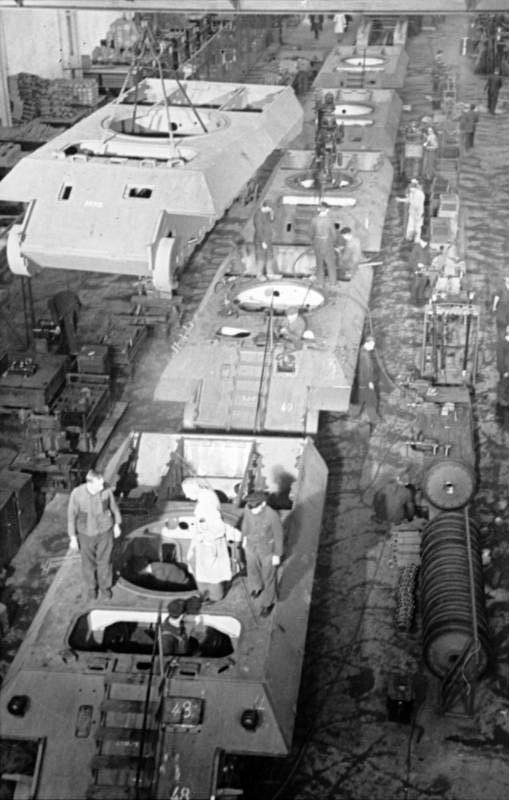
\includegraphics[height =.6\textheight,width=.4\textwidth]{figuras/fabrica_tanques.jpg}
\caption{Ações paralelas, distribuídas, concorrentes ... e tudo planejado!}
%\label{ag_01}
\end{figure}
    
   
\end{frame}





%------------------------------------------------------------------------


\begin{frame} %[allowframebreaks=0.9]


\frametitle{IA Distribuída}

\begin{itemize}
  \item Entidades (ou várias) que interagem sob uma:
  \begin{itemize}
    \item Organização (há uma conexão entre as partes)
     \item Ação 
     \item Interação
  \end{itemize}

     \item Metáfora usada de inteligência: \textcolor{blue}{\textbf{comportamento  social}} (sim, os dos seres animais, incluindo o \textit{homo-sapiens}!)
\end{itemize}


\end{frame}

%------------------------------------------------------------------------

\begin{frame} %[allowframebreaks=0.9]


\frametitle{Resumindo a IAD}

\begin{itemize}
    \item Não é IA paralela (esta é voltada em paralelizar computacionalmente as implementações em IA), nem Sistemas Distribuídos. 
  
    \item Um resolução grupal de problemas, através de  \textit{cooperação} (diferente de \textit{colaboração}).
    
    \item Grande interatividade e capacidade de comunicação.

     \item Organização - meios que garantam a \textit{convergência}: 
      estruturas de autoridade e controle divididos. 

     \item Divisão de conhecimento (nota: \textit{o que é conhecimento?}) e recursos
     
\end{itemize}


\end{frame}

%------------------------------------------------------------------------


\begin{frame} %[allowframebreaks=0.9]


\frametitle{IA Distribuída: 
dois tipos de sistemas}

\begin{itemize}

  \item Resolução Distribuída de Problemas (RDP)
  \begin{itemize}
    \item consciência do objetivo global e divisão clara de tarefas
     \item Exemplos: robótica clássica, busca na Web, gerência de sistemas distribuídos, ...
  \end{itemize}
 
 \item Sistemas Multiagentes (SMA)
    
     \begin{itemize}
       \item não consciência do objetivo global e nem divisão clara de tarefas
       \item Exemplos: n-puzzle, futebol de robôs, balanceamento de carga, robótica, ...

     \end{itemize}

     \end{itemize}
\end{frame}


%------------------------------------------------------------------------


\begin{frame} %[allowframebreaks=0.9]


\frametitle{Porque usar a metáfora de agentes?}

\begin{itemize}
  \item Fornece metodologias de desenvolvimento de sistemas  inteligentes estendendo as de engenharia de software
   \item Fornece visão unificadora das várias sub-áreas da IA 
  \item  Ajuda a embutir a IA em sistemas computacionais 
tradicionais
  \item  Permite tratar melhor a interação com ambiente 
  \item Permite tratamento natural da IA distribuída (distribuir!!!)
  
\end{itemize}


\end{frame}
%------------------------------------------------------------------------


\begin{frame} %[allowframebreaks=0.9]


\frametitle{Ainda RDP $\times$ SMA }

\begin{block}
  
  \begin{description}
    \item[RDP:] 
    \begin{itemize}
      \item Um grupo de especialistas
      \item Habilidades Complementares
      \item Organização Fixa
    \end{itemize}
    
    \item[SMA:]
    
    \begin{itemize}
      \item Agentes podem preexistir
      \item Organização varia em tempo de execução
    \end{itemize}
     
  \end{description}
   
\end{block}

\end{frame}

%------------------------------------------------------------------------


\begin{frame} %[allowframebreaks=0.9]

\frametitle{Fechando esta relação ... RDP $\times$ SMA }

\begin{block}
  
  \begin{description}
    \item[RDP:] 
    \begin{itemize}
      \item RDP é um subconjunto de SMA
      \item Agentes benevolentes, concebidos em conjunto
    \end{itemize}
    
    \item[SMA:]
    \begin{itemize}
      \item SMA é base para RDP
      \item Implementação descentralizada de várias propriedades
    \end{itemize}
     
  \end{description}
   
\end{block}

\end{frame}

%------------------------------------------------------------------------

%------------------------------------------------------------------------


\begin{frame} %[allowframebreaks=0.9]

\frametitle{Um Sistema Multiagente (SMA) formal}

\begin{block}{Um SMA é um sistema que possui os seguintes elementos:}
  \begin{itemize}
    \item Um ambiente: $E$
    \item Um conjunto de objetos: $O$
    \item Um conjunto de Agentes: $A$ ($A\subseteq O$)
    \item Um conjunto de relações $R$, a qual estabelece
    conexões entre os objetos
    \item Um conjunto de operações: $O_p$
    \item Operadores que representam os resultados das operações em $O_p$
     e as reações do ambiente a eles.
       
  \end{itemize}
   
\end{block}

\textcolor{red}{Construa uma tupla para esta formalização}


\end{frame}



\begin{frame} %[allowframebreaks=0.9]

\frametitle{Isto é:}

\begin{block}{Um SMA:}
  \begin{itemize}

   \item Consiste de uma coleção de componentes autônomos, com objetivos particulares
    \item Que se interrelacionam

\begin{itemize}
  \item De acordo com uma Organização
  \item Interagindo, negociando  e coordenando esforços para resolver tarefas 
  \end{itemize}  
  \end{itemize}
   
\end{block}

\end{frame}

%------------------------------------------------------------------------

\begin{frame} %[allowframebreaks=0.9]

  \frametitle{Exemplos de uso de SMAs:}
        
\begin{figure}[!ht]
\centering
%\includegraphics{}
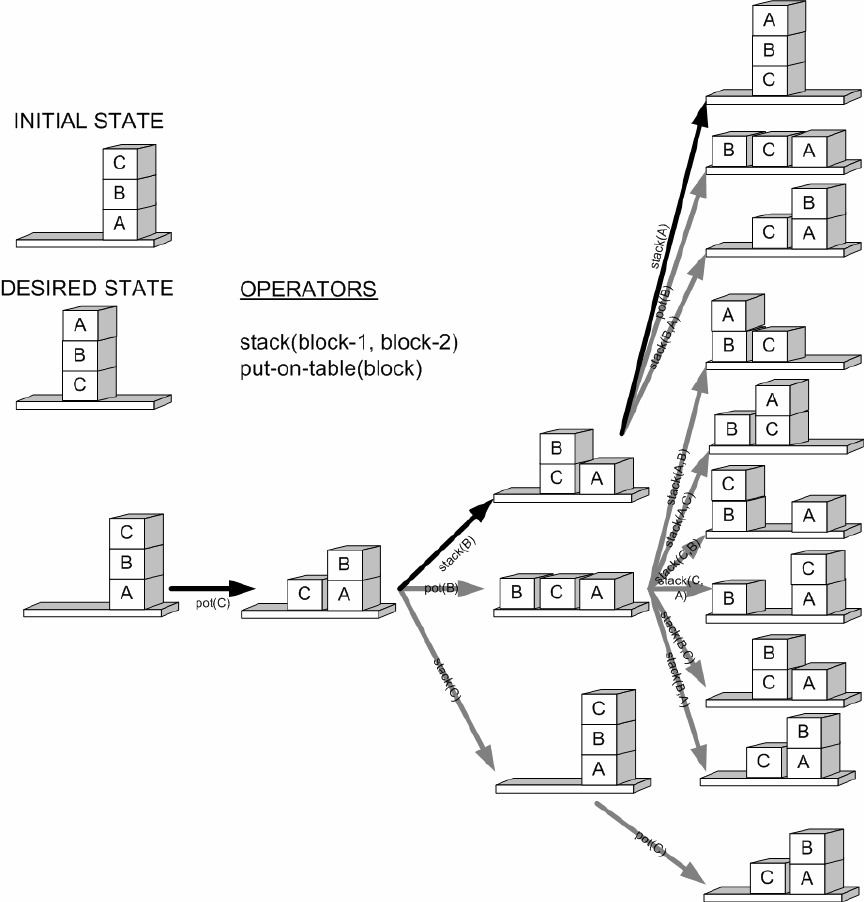
\includegraphics[height =.6\textheight,width=.7\textwidth]{figuras/original_example_SMAs01.jpg}
\caption{\textit{Mundo dos blocos} -- um agente neste caso é previsível}
%\label{ag_01}
\end{figure}
    
\end{frame}

%------------------------------------------------------------------------

\begin{frame} %[allowframebreaks=0.9]

  \frametitle{Exemplos de uso de SMAs:}
        
\begin{figure}[!ht]
\centering
%\includegraphics{}

\includegraphics[height =.5\textheight,width=.7\textwidth]{figuras/example_SMAs01.jpg}
\caption{\textit{Mundo dos blocos} com vários robôs}
%\label{ag_01}
\end{figure}
    
\end{frame}

%%---------------------------------------------------------------------
\begin{frame} %[allowframebreaks=0.9]

  \frametitle{Exemplos de uso de SMAs:}
        
\begin{figure}[!ht]
\centering
%\includegraphics{}
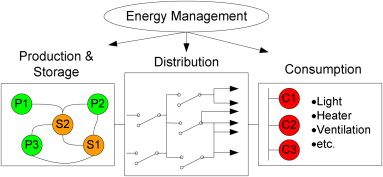
\includegraphics[height =.6\textheight,width=.7\textwidth]{figuras/example_SMAs02.jpg}
\caption{As chaves comutadoras são agentes?}
%\label{ag_01}
\end{figure}
    
\end{frame}
%%---------------------------------------------------------------------

\begin{frame} %[allowframebreaks=0.9]

  \frametitle{Exemplos de uso de SMAs:}
        
\begin{figure}[!ht]
\centering
%\includegraphics{}
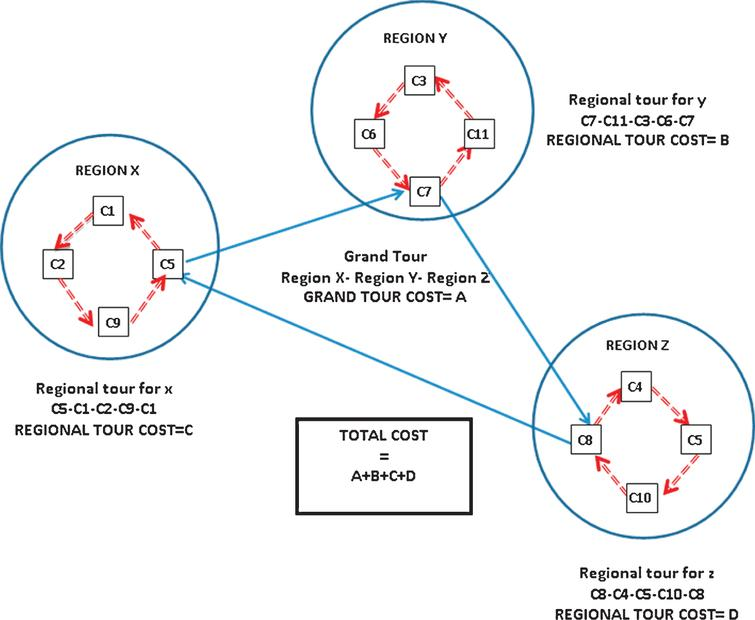
\includegraphics[height =.6\textheight,width=.7\textwidth]{figuras/example_SMAs03.jpg}
\caption{Removendo a dinâmica das regiões este é um exemplo de RDP}
%\label{ag_01}
\end{figure}
    
\end{frame}
%%---------------------------------------------------------------------


%%---------------------------------------------------------------------
\begin{frame} %[allowframebreaks=0.9]

\frametitle{Em resumo... é uma boa idéia quando...:}


\begin{itemize}
  \item Precisamos manter a autonomia das sub-partes
  \item As interações são complexas
  \item Não é possível descrever o problema \textit{a priori}.
\end{itemize}
\end{frame}

\begin{frame} %[allowframebreaks=0.9]

\frametitle{E as  vantagens...:}

\begin{block}{}
\begin{enumerate}
  \item Maior rapidez na solução dos problemas
  \item Diminuição do \textit{overhead} de comunicação
  \item Maior flexibilidade
  \item Aumento da segurança -- tolerância a falhas
\end{enumerate}

\begin{itemize}
  \item \textcolor{blue}{Uma vez definidos e motivados, agora faltam os detalhes 
de como implementar tudo isto!}

 \item \textcolor{blue}{Ver seção de projetos de SMAs!}

\end{itemize}
\end{block}

\end{frame}


%------------------------------------------------------------------------

\begin{frame} %[allowframebreaks=0.9]

  \frametitle{Epílogo: um agente já tem uma realidade \textit{complexa}:}
        
\begin{figure}[!ht]
\centering
%\includegraphics{}
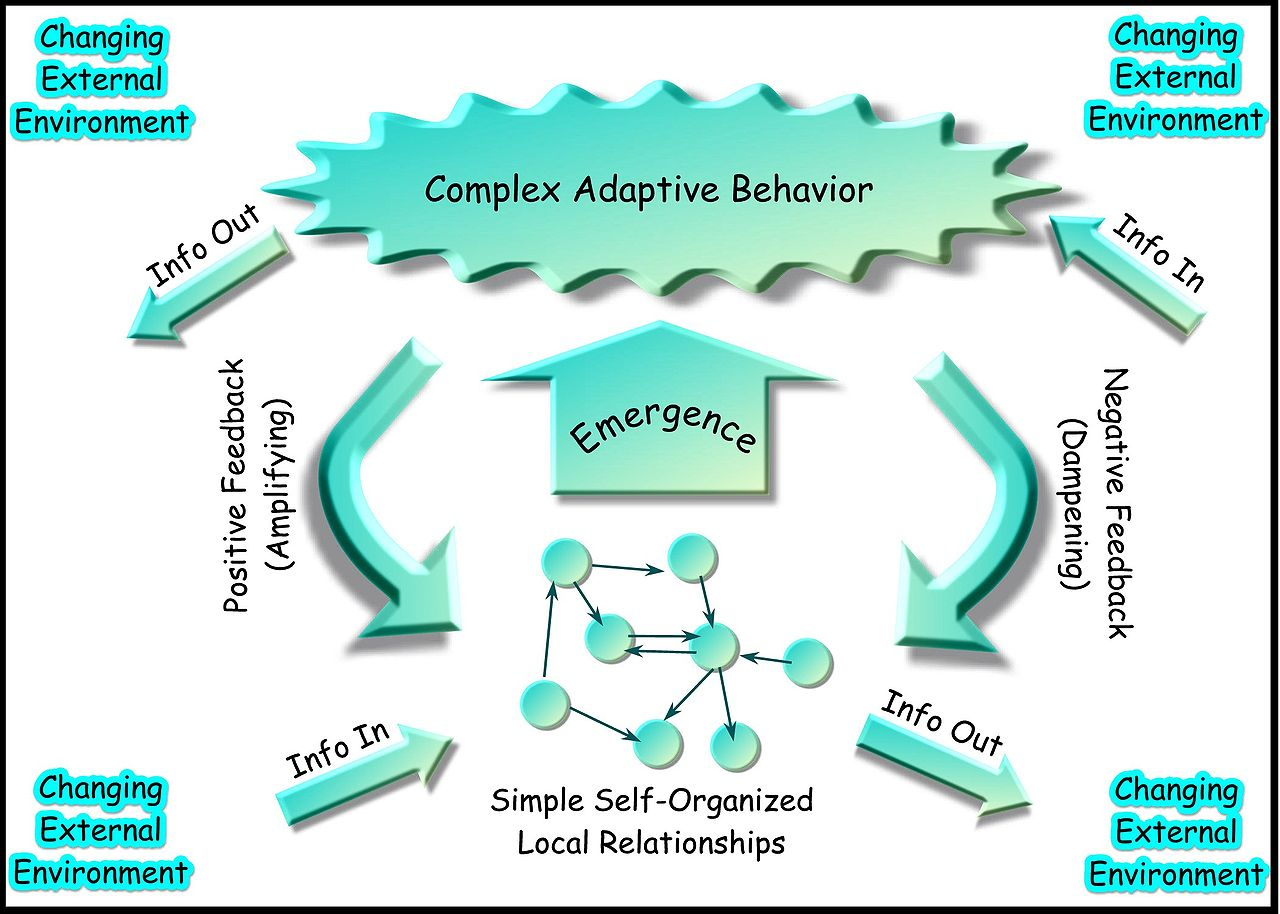
\includegraphics[height =.6\textheight,width=.7\textwidth]{figuras/complex-adaptive-system.jpg}
\caption{Um agente e sua \textit{sociedade de agentes} ...}
%\label{ag_01}
\end{figure}
    
\end{frame}








\begin{frame} %[allowframebreaks=0.9]

 \frametitle{Resumo do capítulo}

\begin{enumerate}
  \item Vocabulário
 \item Diferença de SMAs com RDPs  na IAD
  \item Soluções de SMAs são atrativas porquê
    
    \item Falta: Coordenação etc
        \item Falta: Planejamento etc
     \item Falta: projetar  SMAs     
  
\end{enumerate}


\end{frame}
 % cap 3

\section{Teoria de Jogos, Coordenação e Planejamento}
\begin{frame}

\begin{center}
{\huge Capítulo 4 -- Teoria de Jogos e  Coordenação}

3 partes fundamentais:

\begin{enumerate}
  \item Teoria de Jogos
  \item Coordenação
  \item Planejamento
\end{enumerate}
Nesta ordem
\end{center}

\end{frame}

%-----------------------------------------------------------


%-----------------------------------------------------------


\section{Estratégias de Jogos}
\begin{frame}

    \frametitle{Teoria de Jogos}
    \begin{itemize}
    \pause
      \item 
\pause
      \item 
    
    \end{itemize}
\end{frame}


%-----------------------------------------------------------



\subsection{Teoria de Jogos Aplicado a SMA}
\begin{frame}

    \frametitle{Teoria de Jogos Aplicado a SMA}
    \begin{itemize}
    \pause
      \item $\prod^{n}_{x=1} \neq  \prod_{x=1}^{n+1}$
      \item  \url{https://www.codecogs.com/latex/eqneditor.php}
      \item \url{http://www.hostmath.com/}
      

      \pause
      \item 
    
    \end{itemize}
\end{frame}

%-----------------------------------------------------------

\section{Coordenação}


\begin{frame}
\frametitle{Coordenação}



\end{frame}


%-----------------------------------------------------------


\subsection{Jogos de Coordenação}

\begin{frame}
\frametitle{Jogos de Coordenação}

pag 23


\end{frame}


%-----------------------------------------------------------
\subsection{Convenção Social}

\begin{frame}
\frametitle{Convenção Social}

pag 24


\end{frame}
%-----------------------------------------------------------

\subsection{Papel Social}

\begin{frame}
\frametitle{Papel Social}

pag 25


\end{frame}



%-----------------------------------------------------------
\subsection{Grafos de Coordenação}

\begin{frame}
\frametitle{Grafos de Coordenação}

pag 26


\end{frame}
%-----------------------------------------------------------


\subsubsection{Coordenação por Eliminação de Variáveis}

\begin{frame}
\frametitle{Coordenação por Eliminação de Variáveis}

pag 28


\end{frame}
%-----------------------------------------------------------


\subsubsection{Coordenação por Troca de Mensagens}

\begin{frame}
\frametitle{Coordenação por Troca de Mensagens}

pag 28


\end{frame}
%-----------------------------------------------------------

\section{Planejamento}


\begin{frame}
\frametitle{Fundamentos de Planejamento}



\end{frame}
%-----------------------------------------------------------


\subsection{Abordagens ao Planejamento Multiagente -- SMAs}

\begin{frame}
\frametitle{Abordagens ao Planejamento de SMAs}

\begin{block}{}
 
\begin{itemize}
  \item Coordenação central: controla todos os subplanos
  \item Esquemas de controle distribuído\\
        Conhecimento parcial dos planos de outros agentes
  \item Planejamento Global Negociado

\begin{itemize}
  \item Compartilhamento de todos os planos
  \item Ajuste local para a realização de objetivos comuns

\end{itemize}

\item Modelagem Explícita da Equipe de Agentes
\begin{itemize}
  \item Compromissos conjuntos
   \item Crenças, desejos e intenções comuns

\end{itemize}
\end{itemize}
\end{block}

\end{frame}

%-----------------------------------------------------


\subsection{Exemplos de Coordenação SMAs}

\begin{frame}
\frametitle{Exemplo de Coordenação SMAs}

\begin{figure}[!ht]
\centering
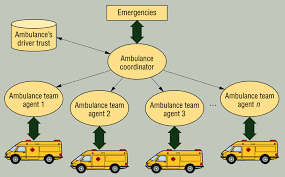
\includegraphics[height =.6\textheight,width=.7\textwidth]{figuras/coordenacao_agentes01.png}
\caption{Coordenação de agentes $\equiv $   SMA}
%\label{ag_01}
\end{figure}
 \end{frame}

%-----------------------------------------------------------

\begin{frame}
\frametitle{Exemplo de Coordenação SMAs}

\begin{figure}[!ht]
\centering
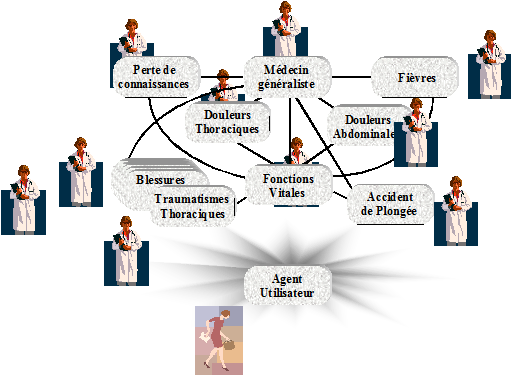
\includegraphics[height =.6\textheight,width=.7\textwidth]{figuras/coordenacao_agentes02.png}
\caption{Coordenação de agentes $\equiv $   SMA}
%\label{ag_01}
\end{figure}
 
\end{frame}


%-----------------------------------------------------------
 % cap 4



\section{Projetos de SMAs}

\begin{frame}

\begin{center}
{\huge Capítulo 5 -- Projetos de SMAS}
\end{center}

\end{frame}


%------------------------------------------------------------------------
\begin{frame} %[allowframebreaks=0.9]


\frametitle{O que vai ter neste capítulo}

\begin{itemize}
  \item Alguma metodologia?
  \item Ambiente simulado: SIM (implementar)
  
  \item O que considerar na construção de SMAs
  \item Perspectivas: reais e visionárias
\end{itemize}


\end{frame}

%-----------------------------------------------------------------------------------

\section{Implementação de SMAs}
\begin{frame}

    \frametitle{Agentes: Metodologia de desenvolvimento}
    \begin{itemize}
    \pause
      \item Decompõem o problema em: \\
      percepções, ações, objetivos, ambiente e outros agentes
\pause
      \item Decompõem tipo de conhecimento em:
      \begin{itemize}
        \item Quais são as propriedades relevantes do mundo?
        \item Como o mundo evolui?
        \item Como identificar os estados desejáveis do mundo?
        \item Como interpretar suas percepções?
        \item Quais as conseqüências de suas ações no mundo?
        \item Como medir o sucesso de suas ações?
        \item Como avaliar seus próprios conhecimentos?
    
      \end{itemize}
      
      \item O resultado dessa decomposição indica a arquitetura e o método de resolução de problema (raciocínio)
      
    \end{itemize}
\end{frame}

%-----------------------------------------------------------------------------------

\subsection{Simulação de Ambientes}
\begin{frame}

\begin{block}{Em geral a construção do agent segue um programa tal como:}
  

  funcao simulaAmbiente (estado, funcaoAtualizacao, 
                         agentes, final)
repita
	para cada agente em agentes faça
		 Percept[agente] := pegaPercepcao(agente,estado)
	para cada agente em agentes faça
		 Action[agente] := Programa[agente] (Percept[agente])
      estado := funcaoAtualizacao(acoes, agentes, estado)
	  scores := avaliaDesempenho(scores,agente,estado) 
	            opcional
ateh\_final

  
 \textcolor{red}{ Cuidado para não cair em tentação e ''\textit{roubar}” \/ do ambiente a descrição do que aconteceu. Usar a memória do agente!}
 
 
 
\end{block}  
    
  
\end{frame}
%-----------------------------------------------------------------------------------

\begin{frame}
\frametitle{Desenvolvendo um agente inteligente:}
\begin{block}{}

\begin{description}
  \item[Projeto]
  
  \begin{itemize}
    \item Modelar tarefa em termos de ambiente, percepções, ações, objetivos e utilidade
    \item Identificar o tipo de ambiente
    \item Identificar a arquitetura de agente adequada ao ambiente e tarefa
  \end{itemize}
  
  \item[Implementação]
   
   \begin{itemize}
     \item O simulador de ambientes
     \item Componentes do agente 
     \item Testar o desempenho com diferentes instâncias do ambiente
   \end{itemize}
      
\end{description}

\end{block}  
 
\end{frame}
%-----------------------------------------------------------------------------------

\begin{frame}

    \frametitle{Simulação de Ambientes}

     ESTRUTURAS ... ver NORVIG -- pg 34 da T

\end{frame}
%----------


%-----------------------------------------------------------------------------------

\begin{frame}

    \frametitle{Simulação de Ambientes}

     ESTRUTURAS ... ver NORVIG -- pg 34 da T

\end{frame}
%-----------------------------------------------------------------------------------








\begin{comment}
\sectio{Aprendizagem}
\begin{frame}

    \frametitle{Aprendizagem}
    \begin{itemize}
    \pause
      \item 
\pause
      \item cap 7
    
    \end{itemize}
\end{frame}
\end{comment}
 % cap 5

%%%%%%%%%%%%%%%%%%%%%%%%%%%%%%%%%%%%%%%%%%%%%%%%%%%%%%%%%%%%%%%%%%%%%

\section{Conclusões}

\begin{frame}

\begin{center}
{\huge Capítulo 6 -- Conclusões}
\end{center}

\end{frame}

%%%%%%%%%%%%%%%%%%%%%%%%%%%%%%%%%%%%%%%%%%%%%%%%%%%%%%%%%%%%%%%%%%%%%
 % cap 6

\end{document}
